%% LaTeX document class.
%!TEX program = htlatex
\documentclass[medieteknikk]{gucmasterthesis}
\usepackage{ifpdf}
\ifpdf
\usepackage[pdftex]{graphicx}
\usepackage{epstopdf}
\else
\usepackage[dvips]{graphicx}
	\usepackage[dvips]{hyperref}    % For cross references in pdf
	\fi
	\usepackage[final]{pdfpages}
	\usepackage{mdwlist}
	\usepackage{url}
	\usepackage{float}
	\usepackage{todonotes}
	\usepackage{hyperref}
	\usepackage{listings}
\usepackage[utf8]{inputenc}     % For utf8 encoded .tex files
\usepackage[british]{babel}     % For chapter headings etc.



\begin{document}

	\thesistitle{Obfuscating Malware through Cache Memory Architecture Features}
	\thesisauthor{Caglar SAYIN}
	\thesisdate{\gucmasterthesisdate}
	\useyear{2014}
\makefrontpages % make the frontpages
\thesistitlepage % make the ordinary titlepage


\chapter*{Abstract}

Have you ever realize how secure and safe environment they claim in security product companies' advertisement? Does Anti-Malware software really provide 100 percent security against Malware? As Everybody knows, It is not. Today, it is nothing more than cat and dog fight. Malware authors purpose an new architecture, an new approach and Anti Virus companies just try to fix vulnerabilities. Due to this fact, Parallel and concurrent architectures are elusive field for malware. They are new, trendy, popular, complex. 

In this thesis, we will try to show vulnerabilities on concurrent and parallel cpu schedulers and non-uniform memory architecture. The weaknesses on hardware layer of the computer are hard to be observed by software solution. Therefore; It is time to pay attention for them, since it is not hard to predict that attackers will focus them.

This thesis purpose an offensive security approach, how malware can be evade autonomous malware detection systems, and also purpose and experimental method to detect and mitigate them. 

\chapter*{Preface}

I would like to thank Erik Hjelmås for encouraging me to write this
small \LaTeX\ class for GUC's master's theses, and in particular for
making sure that I will not be responsible for maintaining and
supporting it\dots

\chapter*{Ethical and legal considerations}
\begin{quote}

	"Virus don't harm, ignorance does."\\
	- VxHeaven
\end{quote}

The content of this document could be used in order to malicious purpose, but any matter or information could be misused in the life and ignorance is not known well as a defense strategy. In this purpose, this thesis aims to enlighten security specialist and system developers against recent way of the possible attacks. 

However, in order to act ethical responsibility, we tried to eliminate practice of tools and piece of codes which could leads malicious usage. In any case, there is no doubt that it is critical to discover and publish vulnerabilities which could cause deep impact before malicious people discover and abuse them.

\todo[inline]{rewrite here}

\vspace{\baselineskip}
\noindent Ivar Farup, \gucmasterthesisdate
\tableofcontents
\listoffigures
\listoftables
\chapter{Introduction}
The purpose of introduction chapter is giving the readers blueprint of the subject, the problems that we face, the change in the solutions, as well as motivation of its importance. In addition, It also purpose to form proper research question which will guide thesis. 

\subsection{Topic covered by the project}
The thesis purposes an architecture of the malware which process parallel, access memory concurrently, conceal itself systematically, shortly that it is likely to be rocket science. However, everything actually started with a simple mathematical theory by John Von Neumann \cite{von1966theory} and the first example of practical malware is written by Bob Thomas at BBN, and it was called Creeper 

The malware is abbreviation of malicious software. It could be any piece of code which is defined malicious. There is no formal definition of malicious, it could be some software advertise without any contest or it could be self-producing code piece which aim to distribute itself and steal your private information, and it turned an arm race between power holders today.

With development of the first malware, their counter software are created and anti malware software have evolved with them so far. In this race, malware authors are always one step further, because of security's nature. This race between black and white side raised the bar above. The motivation of the information amount and severity influence both today, and that information can be sometimes vital. 


\subsection{Keywords}
Security, Concurrent Malware Design, Malware, Multi-processing Architectures, Parallelism and Concurrency, Cache Oriented Polymorphism, Cache Coherency Problems

\subsection{Problem description}
The one of the main and indecipherable problem in security discipline is formulating general threat definition and recognizing malicious activity and all this problems unsurprisingly reflect on information and computer security concept. Security is defined by system's identification, which involve with purpose, crowd, design structures, network model and so on, and today's information system which is designed with various architectural forms is protected against malware by general purpose protection tools. In the market, The anti malware tools producers focused on pragmatic solutions to survive, but it leads to that most of these tools are utterly reverse engineering process which works on result instead of reason.

With usual and pragmatic signature based methods, there are two mainstream techniques to detect malicious code which are called static and dynamic analysis.Static analysis identifies malware mainly with code flow graph and data flow graph on stored file which is not processing. However, On the dynamic side it is a bit more tricky to analyze process, because you are working on the running pieces of codes without knowledge of structures and worse than this, it must concern race condition and memory coherency flaws.

The detection methods and techniques have been adequately worked so far because of the simplicity of architectures and usage of the massive generic computers, However, with increasing of the not standardized, parallel and popular devices like arm's SoC, it is not hard to estimate their new challenges. It is really likely to evade and obfuscate properly your on-the-fly processes with using uncertain characteristic of parallel processing, complexity of concurrent programming, and structure of “Non Uniform Memory Architecture".


\subsection{Justification, motivation and benefits}
If malware designing is superficially considered, you could fall in usual fallacy that It is not beneficial and exactly opposite. However, if we can design it, there is always more skillful author who already abuse this vulnerabilities on the black side of the moon. The work we are obligated to actually proof this vulnerabilities and design counter measure against them. In this way, our blessed motivation is finding possible vulnerabilities, and mitigate or eliminate their risk. Otherwise; if we confront with unknown attack, it could be too late to fix and analyze it. For example, some of the most sensational and beneficial papers are criticize malware as same as the thesis (\cite{moser2007limits},\cite{cavallaro2008limits},\cite{egele2012survey}), and their values are undoubted today. 

\subsection{Research questions}\label{research:questions}

\begin{enumerate}
	\item Can a malware model be designed with using parallel and concurrent architecture in order to conceal its presence from detection mechanism?
	\item If we can design the mentioned malware, can we build a detection mechanism against these kind of malware's presence?
	\item If we build the detection mechanism, What is detection complexity of the algorithms?
\end{enumerate}


\subsection{Planned contributions}
This Master thesis is looking for better understanding on concurrent malware abilities and their counter-measure. Especially, It will try to show how possible to abuse concurrent memory accessing and how durable recent detection kits. It is quite unique work which we have to consider on the future. Ultimate goal is to eliminate any uncertainties which detection methods encounter with concurrent memory accessing.



\section{Choice of methods}
	This thesis will use a technical approach to the problem. It will use quantitative and model building approach. The methodology consist 8 circular step which are, asking question, building new hypothesis, planning methods, developing software, preparing generic testbed, testing, analyzing, reporting results. In addition to this, the large portion of the time will be given researching related topics, based architecture, and learning tools and technologies. Consequently, the accuracy of the thesis is lies on the proper scientific methodology.

	\todo[inline]{ circular diagram will be Drawn here}


	To address the first question, designing proper malware evasion technique with concurrent and parallel architecture have not been researched well so for, therefore; it will lies on so much experiment and we might have to reflection of other evasion and obfuscation attacks analogy.  We will chose several known malware, which is on air, to  evade them during testing part. We will strong probably use kernel modules and android operating systems for testing bed, however we could linux OS without android layer to simplify and closure test period. In testing step, we will use several anti-virus system such as Avast, Comodo, Norton and compare the result before evasion and after evasion. Testing period might me include mathematical proof depending on evasion or obfuscation method.\todo{Consider involvement of this line during project.} At the end of the each hypothesis` result, which is mean the method for concealing malware, will be reported properly. Each method will be another hypothesis, so we could be proof whether multiple or none successful hypotheses, yet the failed hypothesis could be crucial. There could be also many result which are too baroque to proof them or explain their result, these cases could be observed on further work. For semantic knowledge, we could try to show relationship between evasion methods and hybrid approaches.

	If we can find successful hypothesis for first question, we observe them in second question. Second question is depend on the first question's answer. Second questions methodology is actually exactly same circular. It start with defense hypothesis against evasion method. Dynamic and static detection methods must be both considered. The development of the counter algorithms could be proved mathematically, but it can be quite baroque to formulate it. In order to prove it, we could design evasion and detection methods` Turing model, however; the main approach of our testing is involved with experimental solution. we will develop planned algorithms prototype. Proper test bed could be provided with lots of malware species.. We will test our algorithms` prototype with concealed or obfuscated viruses. If it is really necessary, we could prepare also control groups to prove trustworthiness of method, then we have to record result without any intervention. For semantic knowledge, we could try to show relationship between detection methods and hybrid approaches.
	\todo{depending on the found evasion technique, methodology could be shaped again}
	\newpage

	The last question is a matter of measuring and analyzing algorithms complexity. It is totally mathematical scientific methodology. We have to analyze worst, best and average complexity rate. There are also several Quantitative approaches like measuring resource usage. It could be efficient some system like network which there are lots of uncertainties in.

	In this project, there five inevitable risks which we can face during development.

	\begin{itemize}
		\item The thesis is highly dependent on the hardware, and the cost of the hardware constitute risk on its own. Any case of hardware defect leads to comprise obstacle.
		\item Hardware dependency is also leads to logistical and time consuming risk which could result with latency on submit time.
		\item Firmware codes which we are planning to work on are mostly undocumented. We could discover their usage by proper reverse engineering and fuzzing process when required, however it is obviously manpower.
		\item Most important and highlighting risk is there isn't proper research on this particular area. That means there are strongly possibly hidden risks which could cause other mental and physical result.
		\item During testing and purification part, Anti-malware tools could come out with unreliable result. To analyze result properly, we may need to inspect mentioned tools with reverse engineering process which could violate proper usage agreement. To mitigate that kind of risks, we could request research agreement from companies.  
	\end{itemize}



%!TEX root = thesis.tex
\chapter{Related Works}
\section{Malware Self-Defense}
This section will give an overview of researches about Malware`s self-defense technique, the methods to analyze them, and their application on concurrent architecture. 
This section will try to give the literature about malware evasion techniques. This techniques are generally antonym solution which are found by malware authors, however, there are enough surveys about known technique. We classified all these methods in six categories which are code obfuscation, code reuse, anti debugging, anti emulator and visualization and covert channel over network traffic. This taxonomy is well defined by Jonathan A.P Marpaung, et al \cite{marpaung2012survey}, yet malware authors used them to protect their own properties. 


Code obfuscation was originally  found for protecting intellectual property\cite{balakrishnan2005code}, but It aims to puzzle code`s binary against merely static analysis and disassembling\cite{nachenberg1996understanding}. The first known obfuscation method used encryption in order to hide its content. It was called Cascade which is seen first 1986\cite{you2010malware}. This simple architecture of the obfuscation is called packing\cite{internotsecurityteam}. It involve with two part of binary which are slub part, in order to decipher and encipher.\cite{marpaung2012survey}. Cascade was using simple XOR encryption and that was increasing performance.

Early of the 1990s , oligomorphism and polimorphism started to show up\cite{you2010malware}. The main idea behind them is basicly transforming their slub part in each attempt of encryption process\cite{nachenberg1996understanding}. Today, there are two type of  polymorphic approach to generate different variants of slub.\cite{li2011mechanisms}
\begin{itemize}
  \item Rewriting the code each time from pseudo-code so it differs code synthetically which is actually transformation based obfuscation.
  \item Self-cipher itself different, order of these ciphers and using different keys.
\end{itemize}
One of the other important milestone of polymorphic malware is Mutation Engine(MtE) is writen by a Bulgarian virus Author, called The Dark Avanger. It was automated obfuscation tool which actually considered impossible in those times.\cite{anonymous1}

There are also several methods to prevent unpacking process. These methods are collected carefully by Peter Ferrie \cite{ferrie2008anti}. These methods are especially obstacle for automated analysis.

Compare with polymorphic methods, metamorphic approach is more complicated. It is transformation based method instead of encryption  approach.\cite{konstantinou2008metamorphic} Fundamentally, it produce different codes which doing same blue printed semantic. That just mitigate detection possibility because of lack of static code. 

Network traffic, which malware produce are generally Achilles heel for malware, because they are generally adequately unique traffics to be identified\cite{marpaung2012survey}. They usually cover their overt malicious traffic with covert channel methods.\cite{rutkowska2006rootkits}

Code reuse attacks are strong attacks because they do not inject any code in them as obfuscation methods did. They aim to use legitimate software to evade themselves. There are there well known applied version which are return-into-libc, return oriented programming and Frankenstein.

Return into libc attacks were demonstrated by solar designer in 1997 as a method of bypassing non executable stack to executable libc libraries\cite{designer1997getting}. It's object is to change the "ret" infrastructure argument to the known address possibly libc library(stdio, system, etc). However, this attack is limited with libc libraries, which we improved with return oriented programming. 

Return oriented programming is more flex version of retur-into-libc attack, which is introduced by Shacham in 2007\cite{shacham2007geometry}. Return oriented programming purpose a programming language with small gadgets(instruction bound) which involve all ability of Turing's machine\cite{roemer2012return}. Frankenstein is one of the novel application of return oriented programming by Vishwath Mohan and Kevin W. Hamlen\cite{mohan2012frankenstein}.

Anti debugging and anti emulator methods are really usual for today's malware. The survey of Chen Xu et al. showed us in 2008, majority of 6900 on-the-air malware could evade their self with exhibiting benign behavior in sandboxes, debuggers, and virtual machines.\cite{chen2008towards}. VM and debuggers are most important element of dynamic analysis techniques in autonomous sector, because it must run the file just before it touch the working environment. Yet, it is not that knotty to determine whether working environment is virtual or not. Fuzzing cpu bechmarks and comparing results entropy is a good way to determine virtual machines.\cite{franklin2008remote}

Rootkits are the piece of malicious code which aims to crack integrity of the system state. The idea of the remaining invisible to the system state is traced backed one of the oldest virus "Brain"\cite{martin2008}. It was changing the boot process and activate virus during booting. "Tequila" and "1689" viruses followed "Brain" in 1991 and 1993\cite{Ducklin1991}. There are NTRootkit and HackerDeffender rootkits today. The proper classification of the rootkit are prepared by Adnan Abdakka\cite{Adnan2011}.



\section{Malware analysis methods}

\begin{figure}[h]
    \centering
    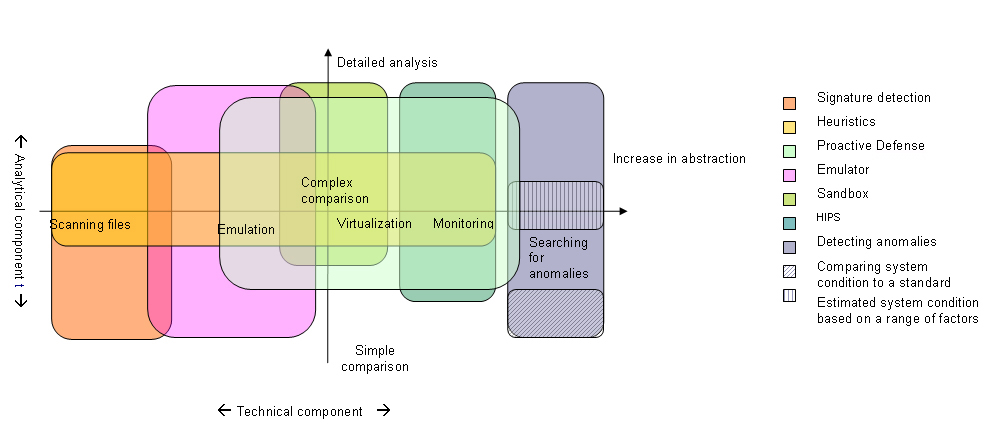
\includegraphics[width=1\textwidth]{img/alisa_1007_pic1_en.jpg}
    \caption{Detection models \cite{Shevchenko2007detc}}
    \label{fig:awesome_image}
\end{figure}
Malware analysis medhods could be considered two dimensional plane which are "anomaly, signature based detection technique" and "Statistic and dynamic analysis method". 



There are also several applied techniques, which combine terminology above. 
\begin{description}
\item[N-gram] It is a anomaly  based heuristic detection method algorithm. It is a bit costly process and not practical for client side analysis. It could be fit for honey pot analysis \cite{reddy2006n} \cite{abou2004n} \cite{abou2004detection}. They are capable against to zero time malwares and that could makes it futures malware detection system. 
\item[Sequential approach on system and funtion call] This approach is anomaly based dynamic analysis and observing and recording the flow graph of systems and function calls and  try to analysis anomaly behaviors.\cite{kendall2007practical}
\item[Taint] It is also called data flow analysis or data flow graph. It is basic tracking marked data values during execution.\cite{saxena2008efficient}\cite{saxena2008efficient}\cite{smith2007principles}
\item[Control Flow Graph] They are one of the most important arm of commercial autonomous malware detection tools\cite{lee2010detecting} \cite{christodorescu2006static} \cite{christodorescu2005semantics}. After the invention of the polymorphic and metamorphic, syntactic analysis could not bear with them. Then we moved to upper layer of information, semantic layer. Semantic can be representation of code flow, and the routes of the code are adequate to produce signature to identify malware. This methods are a member of static analysis and disassembling and source code analysis job.
\item[Network Monitoring] Malware intention of the communication over network actually big clue to detect them. They generally use unique hostname, ip adress or specific protocol with particular way \cite{marpaung2012survey}.
\end{description}
%!TEX root = thesis.tex
\chapter{Background Studies}
\section{Caches}
Solely, a cache is a small, fast, array of memory which is placed between lower level memory and higher one.  It store a special block of information, in order to increase performance of computer systems. It is like a buffer area which has some logic to exploit locality features of programming logic. Today, with increasing of processing ability of computer systems, memory access is bottle neck. 

The "cache" is originally french rooted with meaning "concealed place for storage."\cite{sloss2004arm} We can move this definition basically to the computer science. The cache's design is definitely  isolated from software layer, however; if you know your caches feature and how caches working you could program a lot more efficient codes easily.



\subsection{Motivation of Caches and Principle of Locality}
The main motivation of caches is indisputably performance. As we mentioned,  Performance of high-speed computers is usually limited by memory bandwidth and latency. In order to increase, and turn around that, we use an small array of memory which is located close to the processors.  The location of chip is important and there are many design decision (e.g On chip, out of chip), but more crucial  properties of caches are their designs (e.g. Naive Capacitor , SRAM, DRAM) and their logic complexity\cite{hennessy2012computer}.Due to physical constrains, the size of the memory is limited which we can locate close to memory. On the other hand, these design choices are decisive factor about prices of memories.  Because of all these reasons, Multi-Layer Memory Hierarchy with several caches  between processor core and main memory is well-known option in order to improve performance. Nevertheless, In multilayer memory hierarchy, it is hard to know where the particular data reside in, and whether it is coherent or not. It also add many layer between memory and processor and in some cases it even decrease system performance,especially because of logical complexity of the line.

The idea all the caches logic depending on is Principle of Locality. Principle of locality is actually a concern of information theory\cite{shannon2001mathematical}. It a conjecture of data distribution and processing order. The phenomenon assume that the the same data and related document will be accessed more frequently than other data\cite{denning2005locality}. Today, it is the one of the corner stone of computer science.  It was first developed with Atlas System with purpose to develop virtual memory systems work well\cite{kilburn1962one}. Then, it spread from search engines optimization to hardware caches. 

\begin{figure}[h!]
    \centering
    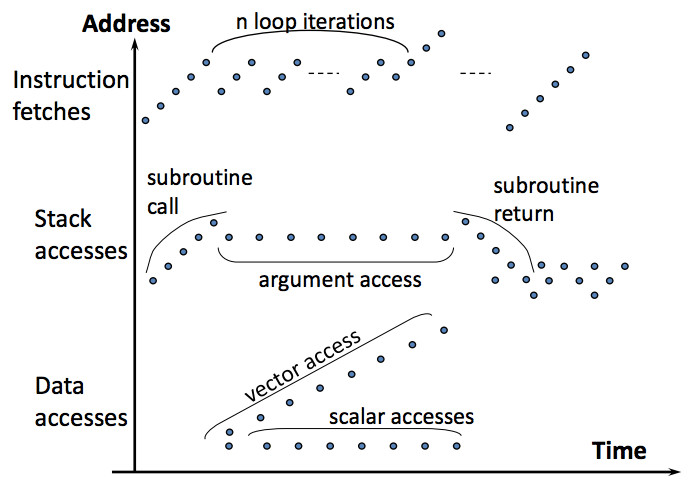
\includegraphics[width=1\textwidth]{img/localitygraph2.jpg}
    \caption{Principle of Locality}
    \cite{ComputerArchCoursera}
    \label{fig:principleoflocality}
\end{figure}


There are mainly two type of locality of reference:

\begin{description}
\item[Spacial Locality] Spacial locality propose if there is a particular of memory which is accessed on memory, then it is more likely to accessing memory locations around of it in near feature. Especially arrays and instructions are exploiting this locality. Arrays, formed structure and instructions on memory are laid out lineally over memory. On figure \ref{fig:principleoflocality}, we can see spacial locality simply.  For example, during instruction fetches part on the figure, n loop iterations accesses same memory locations for many times.  There are also subclass of spacial localities like Branch Locality and Equidistant Locality. They are designed locality types of indeterministic feature of program structure. Branch prediction and Special compiler designs aims to exploits this kind of locality more efficiently.
\item[Temporal Locality] Temporal locality propose if there is a particular of memory location which is accessed recently, it will be accessed again more likely than any other location. Especially, variables, subroutines of stacks or other calls exploits this feature of locality. On figure \ref{fig:principleoflocality}, it is obviously seen that the values accessed once is possible to accessed again. 
\end{description}

\begin{figure}[h!]
    \centering
    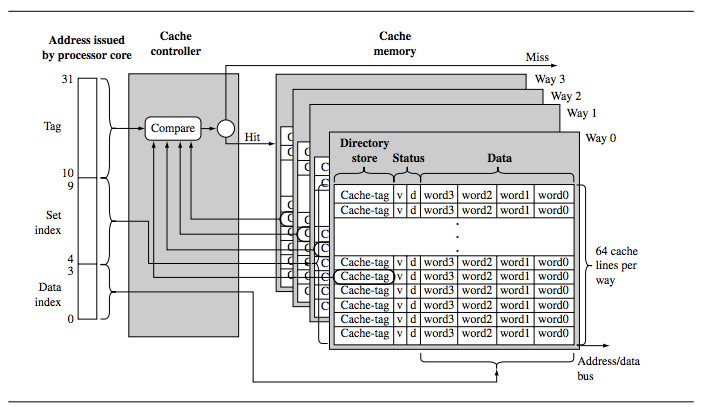
\includegraphics[width=1\textwidth]{img/cacheinternals.jpg}
    \caption{4 KB 4-way set associative cache with 256 cache lines }
    \cite{sloss2004arm}
    \label{fig:cacheinternals}
\end{figure}

\subsection{The basic logic of caches}
As we said in previous section, the basic logic behind caches is moving arranging caches with local data. In order to provide this feature as smooth as possible, we use a logic circuit called "Cache Controller". It does basic logic comparison and wiring the request and response into the right path. Thus, it intercept the write and read request from processor, replace its memory array with right scheduling method, and evict it safely and coherently. It processes with diving address of th request into three fields which are  Index set field, tag field, and block field. In figure \ref{fig:cacheinternals}, these fields showed. 

At the beginning of cache process after it divided address fields, It first request right cache line which is shown in figure \ref{fig:principleoflocality}. So if we have $M$ byte memory and $N$ byte cache line, we must have $M/N = cache line$, then we can represent it with $p$ when $cache line = 2^{p}$ Thus, cache controller just wire corresponding line with given set index. 

In traditional cache convention, first field belongs to tag id. Tag id is determined depending on other field i.e. the remaining part after index field and block field calculated is tag id length. Tag id is using to verify the stored line is actually belongs to right location of memory. The cache controller has comparison circuit(XOR) and compare the requested address and the address which is in the pointed line by set index field. If they are matched with each other, then it check valid byte and hit or miss. There is a simple AND circuit between tag comparison. 

Final field is called data index or block index field. It will point in the cache line the smallest addressable memory location. Therefore, when processor want to read a value, cache fetch the whole block, and that makes cache to exploit spacial locality linearly. However, it will limit the access speed remarkable, if we increase block size. The optimum block size is about 64 byte for many system. As we mention before each cache line includes cache-tag field, valid bit, dirty bit, and some coherency bits in some special systems. The length of the data index field is equal to r if  $ word size = 2^{r}  $.

When we increase the set index count it increase basically temporal locality, but not always. The cache conflict could happened when two memory location which uses same cache line could be used concurrently or twisted. Highly trashing can reduce cache performance. For this reason, associative caches are developed. Set associative caches are represented by their way number e.g 3 way associative caches or full associative caches, and there are group of cache arrays corresponding to the same set index. So that decrease the set index count but increase the performance during conflict miss in some cases. However, because of the complexity of the comparison circuit, it must be carefully chosen the number of ways. The associative caches are showed in figure \ref{fig:cacheinternals}. 

The computer architecture we uses today actually first formulated by John Von Neumann  \cite{von1961collected}. On the first design of computer it was a single cycle instruction machine without any pipeline or superscalar idea. Then Hardward Mark I machine is designed with proposing two type of caches which are one for instruction, and one for data. Icache and Dcache are specified for their own purpose, because data and instruction on memories have different deterministic properties. Instruction are more tent to be linearly accessed by memory and they has branch locality which can be predict earlier. Icache also could be located more close to decode and fetch parts of processors when Dcache are instead closer to memory fetch parts. Yet, the most significant benefit of Harward design is concurrently usage both caches during pipelined architectures. 
\subsection{Allocation, Write and Replacement Policies}
There are three policy type determine a cache behaviours. They are write policy, read policy and reallocate policy. System's performance, coherency, and designs are determined depending on these rules. 

\begin{figure}[h!]
    \centering
    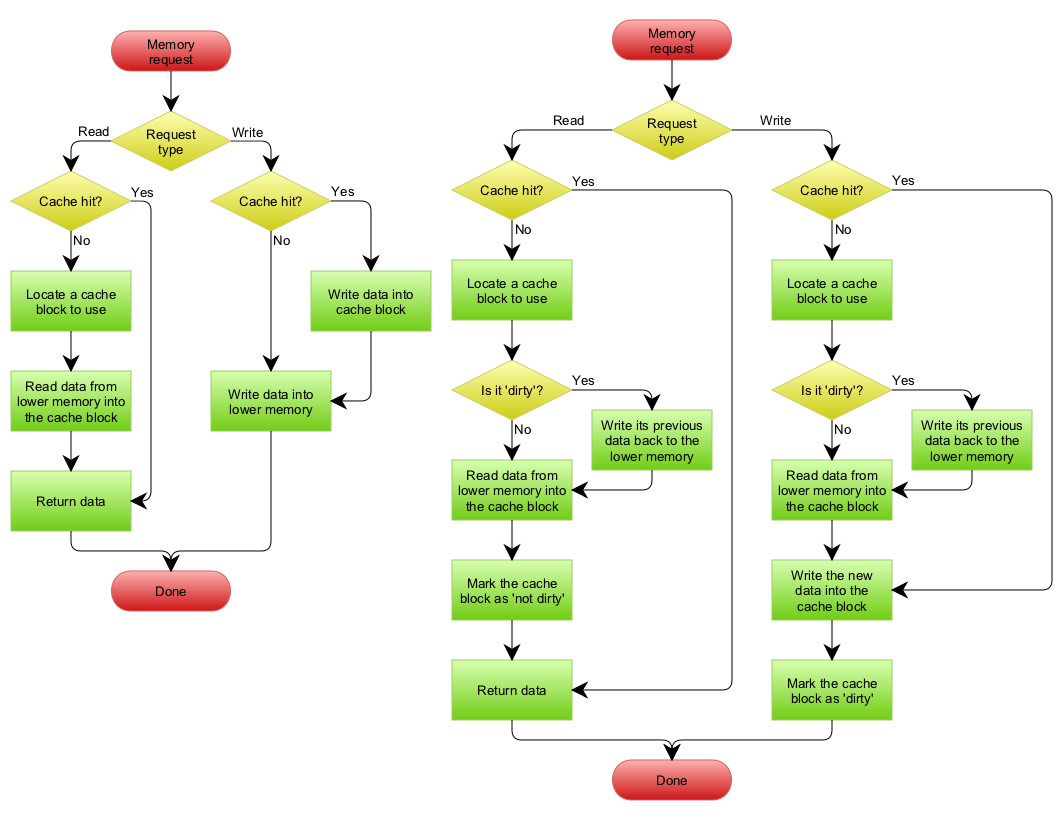
\includegraphics[width=1\textwidth]{img/policies.jpg}
    \caption{A. A Write-Through cache with No-Write Allocation B. A Write-Back cache with Write Allocation}
    \cite{wikipolicies}
    \label{fig:cachepolicies}
\end{figure}

\subsection*{Write Policies }
\begin{description}
\item[Write Through] When the cache controller designed based on $write through$ policy, it write the values into the memory and caches simultaneously, when the write request is arrived from processors. It does not depend on $write miss$ or $write hit$. It will reduce write performance, because writing data on memory is a lot slower, but it stay coherent all the times. It is performance could be increased a bit  with write buffer memories between memory and cache.
\item[Write Back] The systems with that policies does not have same values in memory and corresponding cache line, so the coherency between memory and caches are provided by a trashing algorithm. Cache line always store more recent data, but if there is more than one cache it is hard to decide which one is more valid or whether there is a valid coherent one.  However, it effects performance quite remarkable (e.g. in ARM 15 cpu writing cycle to memory is around 200 cycle, but caches is about 4.) . The system with limited register numbers can overflow to the memory to store loop variables and that could increase write memory usage. $Write Back$ policy makes this kind of systems really effective. The dirty bit are stand for $WriteBack$ policy. If you write some value on any cache line, dirty bit must be set for eviction. During trashing process, you must first move dirt block back to memory. 
\end{description}
\subsection*{Replacement Policies }
\begin{description}
\item[Random] Random policies are designed to evict a random line in the associative caches. It is  not really random on implementation, but enough random to work with it. It sounds to weak and primitive approach but actually it could be really effective on highly associative caches. 
\item[Least Recently Used ] Least recently used replacement policies are actually implemented in two types. Fully most recently used and Not most recently used random. It is probably the most efficient algorithm to replace cache index sets, but it is really hard to implement on highly associative caches. You must record history of schedule and update it each attempt of access. It could be most effective and easy method on 2 way associative caches and it just need one bit to record who used last. It actually increase temporal locality, because it offers the most recently used one is more likely to be used again. The most recently used but random is a hybrid solution of least recently used and random policies. It just record who accessed last and replace one random set except most recently one. 
\item[First In First Out] It is also known Round robin. It is also mostly using with highly associative caches. In its implementation, it has one one tail pointer of stack and in each attempt of access it evict tail pointers set, and increment the the tail pointer to next set. 
\end{description}
\subsection*{Allocation Policies }
\begin{description}
\item[Write Allocate] $Write Allocate$ policy is also known as $Read Write Allocate$ policy. It refers that during write miss process, cache controller allocates the cache line with related address, as like as normal read miss process. It is mostly using with $WriteBack$ policies, because it assume it is more likely to access same data which you write before. 
\item[No-Write Allocate] $No-Write Allocate$ policy is also known $Read Allocate$. It is an exotic implementation of caches. It is generally seen with $WriteThough$ policy. This systems can be special to read privileged and they do not hope to read or write subsequent write(or even read after write.) 
\end{description}

\subsection{Miss Type and Advance Cache Optimization Methods}
\subsection*{Miss Type}
\begin{description}
\item[Cold Misses]  Cold misses are sometimes referred to as compulsory misses . If you never invoke related memory address and if you calling it first time,  You will encounter with that misses. It is natural misses, and really hard to mitigate them. Spacial locality is the one of the method to avoid this misses. As we mention before, when we increase the size of block, it will increase spacial locality.Also before initializing memory, pre-fetching algorithms and branch prediction algorithms can be useful to eliminate this kind of misses. In addition to this, usage of large amount of caches will naturally reduce this misses, but it is side effect of it.
\item[Conflict Misses] Those misses are the one we are able to avoid. Conflict happens in systems set with lower associativity esp. with direct map systems. To reduce this you should increase associativity. In full associative caches, it all conflict misses are avoided. The change of conflict miss is $tagsize/memorysize$.
\item[Capacity Misses] They are also natural misses related with size of the caches. We can not store every information in memory into cache. Those misses are based by definition of caches.  You can't solve it even with perfect replacement algorithm, but maybe you could decrease the rate of capacity miss with pre-fetching.
\end{description}
\subsection*{Advance Cache Optimization Methods}
\begin{description}
\item[Pipelined Caches] As we did in processors, we could divide cache organization in two separate stage which are decode and data. It will increase the writing efficiency because it will increase the bandwidth during subsequent requests. However the clock mechanism will decrease to hit time.  
\item[Write Buffers] Write buffers are small fully associated buffer memories between caches and memories. They effects cache performance because the time between writing values to memory from cache, cache memories must lock if we do not use cache memories. Thus, Cache memories store values to buffer buffer will responsible with writing it. Buffer size is important, when consecutive write operation requested. When buffers is full, it will makes cache lock to get empty.
\item[Multilayer Cache] Multilayer caches are game changer optimization decisions, because when we have level 2 caches, then we could have faster level 1 caches, because it could be smaller and simpler. Namely, we are adding systems higher level caches, in order to, decrease lower level caches miss time penalty and increase the hit response time, but it will decrease lower level caches hit rate. Level 2 or higher caches could be also on-chip (i.e fast as possible) and SRAM, yet lower level caches must always be faster closer and simpler.
\item[Victim Caches] Victim caches are really useful and simple idea for decreasing miss penalty time. It is a buffer memory, fully associative and mostly 4 to 16 cache line. It stores recently evicted lines in it. It means it increase the associativity of recently used lines on other small buffer with cheap and flexible design.
\item[Hardware Prefetching] There are many theoretical pre-fetching method, but there are a few example implemented. The most well known is prefetch the most recently values incremental block line. That targets to increase most recently used ones spacial locality. It is really efficient to applying it, because increasing block depth is expensive job for caches and increase hit time. If you implement one buffer memory, which prefetch next block of block you need, it automatically increase spacial locality. Also compiler based branch prediction methods are good example of instruction prefetching, however, generally, prefethers for instruction caches load all branches to decrease miss rate.
\item[Non-Blocking Caches]
\end{description}
\section{Cache Coherence and  Consistency}
Many modern computer systems with parallel processing ability have support of shared memory in hardware. Shared memory has lots of advantage over message based memory systems.  Each processor could access same address space, read and write them simultaneously with using their own caches. This features has lots of benefit such as; low power consumption, higher performance and lower prices. However, without consistency between processors, parallel processing can not use many advantage of parallel programming. It could be also insecure to use a system without consistency between processors. 

To provide better understanding of shared memory correctness, we defined it in two separate them in two definition, which are consistency and coherency. Consistency provide a definition of memory access rules and how they will act around computer system with store and load operations. When we compare it with coherency model, it must be more simple and easy to understand it. Therefore, it define a correct behaviours of the memory accesses of multiple threads by allowing or disallowing executions. On the other hand Coherency is a way of implementing a control protocol between memories and processors to support and provide consistency. Correct coherency provide a system which programmer or operator of the system can never determine behaviours (misbehaviours or correct behaviours) of caches\cite{sorin2011primer}.

As mentioned, Mention Consistency is try to define to correct shared memory behaviour between many processor in term of loads and stores. It does not have to concern specific hardware issues, such as hardware level pipelines, write buffers, caches, Out-of-order processing schemes etc. However, in the market, there is no hardware provide consistency perfectly, because the reordering store and load operations is regular optimization techniques in out-of-order processors. In addition to out-of-order processors, the multi layer memory architecture makes consistency vague and subtle. Yet, most of the programmers assume memories are completely consistent. There are several level between inconsistent and sequentially consistent memory. 

\todo[inline]{Mention Consistency Application Summery.}

\begin{figure}[h!]
    \centering
    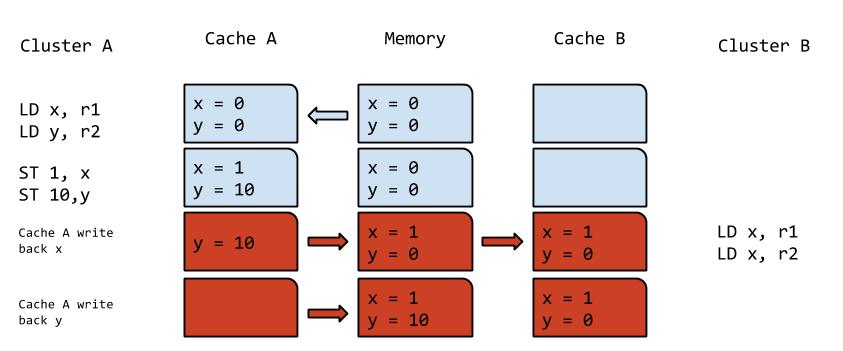
\includegraphics[width=1\textwidth]{img/cacheinconsistencywriteback.jpg}
    \caption{Write-back Policy Cache Memory Inconsistency}
    \label{fig:cacheinconsistencywriteback}
\end{figure}

Memory Coherency (a.k.a. Cache Coherency) is actually to impose a protocol between caches to provide a specific consistency model on shared memory systems. Unlikely consistency, it also concern hardware uncertainness and 
subtle part such as write buffer, pre-fetcher. Typical consistency protocol has features which include instruction caches, multiple-level caches, virtual-physical address transaction, and coherent direct memory access. However, it is not enough to ensure consistency(depending on consistency model) by itself. It tries to makes caches synchronization in shared memory systems invisible from software developer. However there are timing techniques to analysis cache architecture and coherency model of system. 

In figure \ref{fig:cacheinconsistencywriteback} and \ref{fig:cacheinconsistencywritethrough}, the consistency issues on multi layer memory systems. Assume there is two cluster which has ability to process values with given instruction codes. LD and ST instruction refer to memory load and store request. In figure \ref{fig:cacheinconsistencywriteback}, there is a system with two caches which belongs each cluster and one shared memory block. x and y is represents a particular memory address. Contrast with figure \ref{fig:cacheinconsistencywritethrough}, figure \ref{fig:cacheinconsistencywriteback} uses write-back policy. In step 1, cluster A loaded x and y to the processor(it could be also pre-fetcher who load them to the cache block). In second step, somehow clusters stored 1 in memory location x and 10 in memory location y. In this step, memory is not consistent with memory but it is not hazard because they are not shared with cluster B. In step 3, caches evicted the block which include address x and later address x and y were loaded into the cache B. After this moment, they will never share the values which other cluster is actually using. Y was 10 at the end in the memory but it can't be seen by cluster B, even if it try to read it a million times. 


\begin{figure}[h!]
    \centering
    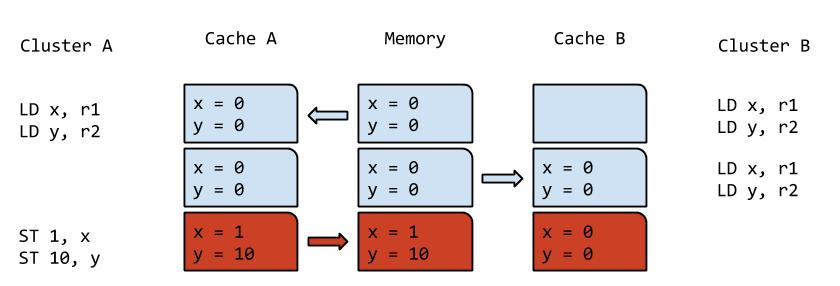
\includegraphics[width=1\textwidth]{img/cacheinconsistencywritethrough.jpg}
    \caption{Write-through Policy Cache Memory Inconsistency}
    \label{fig:cacheinconsistencywritethrough}
\end{figure}

Write-through cache policy is intuitively perceived as solution of this problem, because it just write every values directly to the memory and it will be always synchronized with memory, yet it is not. In figure \ref{fig:cacheinconsistencywritethrough}, write-through cache policy inconsistency showed. The problem with write-through policy, clusters use values which in their cache instead of memory, so even if memory is consistent with clusters, it is not consistent with each caches. In step 1 of figure \ref{fig:cacheinconsistencywritethrough}, cluster A loaded x and y addresses into the its registers. Then, in step 2, cluster B loaded  values of x and y addresses. In step 3, system got in inconsistent state, because cluster A write values through memory, but Cluster B uses the old values, and it will never reach never values, even if it try to load many times. For this reason, many of the large systems which has more than 64 core use this type of cache coherence.

In order to solve this problems, there are several coherency mechanisms and their protocols.  Depending on the case and the number of cluster or processor in the system, system could use Snooping and Directory based mechanism. These each protocol have their own benefits and drawbacks. Snooping protocol is tent to use a lot of bandwidth, however, it is faster and more synchronous. Its logic is to broadcast each state to every node on the system. However, directory based mechanism work with request and response. There is interconnector to forward message to the right address and it makes directory based mechanism slower because of the increased latency, lighter because of the decreased bandwidth.

\subsection{Snooping Coherence Protocols}
Snooping coherence (a.k.a. Bus Sniffing) is a technique to have caches to watch other processors caches and provide consistency depending on specified protocol.  It basically implemented with external port to the system bus. Therefore, it implemented over cache controller which has feature to watch bus. It makes cache controller bigger and waste more power, so lower layer caches could use less complex coherency protocols and vice versa. There are many snoopy cache coherency protocol also depending on consistency model, but we can categorize them in two class which are Write update and write invalidate. 

In this both protocol, we try to get rid of stall data which are in different caches, but it is provided with different logics. Write-update protocol is a broadcast write protocol that in every write attempt, it will write the values into the corresponding cache block but also it broadcast the write message to the every caches on the connected bus. Thus, everyone on the bus which has the ability of interpreting the message of write-update protocol will update stall values with new ones. 

Secondly, Write-invalidate is whenever you write, you invalidate other cache copies and reduce to possibility usage of stall data. Instead of sending whole data block, it just send the tag number and state of the tag. It could effectively be successful, if you have limited bandwidth and power source. Most processor with coherency is today using write-invalidate protocol. However, it is efficient if there a few writer and many reader clusters or processors. Comparing with write-update protocol, if there is many writer, it could be less efficient because of invalidation process validate-invalidate-forward hops.\cite{ComputerArchCoursera}

There are many protocols for both write-invalidate and write-update to maintain coherence, such as MSI, MESI (aka Illinois), MOSI, MOESI, MESIF, write-once, and Synapse, Berkeley, Firefly and Dragon protocol. In this thesis, we will just focus on write-invalidate protocols because of their popularity, but basic principles are same as each other.

\todo[inline]{Mention Serialization of buses}


\subsubsection{MSI - Basic}

\begin{table}[position specifier]
\centering
\begin{tabular}{|c|c|c|c|c|}
\hline 
• & Clean/Dirtiy & Write? & Unique? & Silent Transition to \\ 
\hline 
Invalid & Clean & No & No & - \\ 
\hline 
Shared & Clean & No & No & Invalid State \\ 
\hline 
Modified & Dirty & Yes & Yes & - \\ 
\hline 
\end{tabular} 
\caption{MSI states' properties}
\label{tab:MSItable}
\end{table}


Basic write-invalidate snoopy cache control protocol is MSI (a.k.a Modified-Shared-Invalid protocol). In this model, each cache block has cache tag, and two status bit as same as standard caches, but instead of dirt and valid status bit, MSI cache line has state bits to refer in which state it is. MSI has three state in state machine and they are "Modified", "Shared", "Invalid". two bits can represent four state, so definitely represent three state. The main idea behind this protocol is that one writer and many reader states provide always consistent memory sharing. Therefore, every cache in the system has different responsibilities when they read or write.

\begin{description}
\item[Invalid] Invalid state is exactly same state with standard caches' invalid state. When cache need to access a invalid block, it must act as cache miss, and  be fetched this block again.
\item[Shared] When there is no writer processor on this line, and if  a processor request this line with purpose of read it, it will be in shared state.  It is read-only cache block, and processors are not allowed write without transforming state. The processor also can evict it without writing back to the upper layer memory, because that is for sure, it is clean block.
\item[Modified] It is modified and also modifiable cache block. In a memory coherent system there can be at most one modified cache and all other cache must be invalidated. It is responsible with writing back cache to the upper layer memory. 
\end{description}


\begin{figure}[h!]
    \centering
    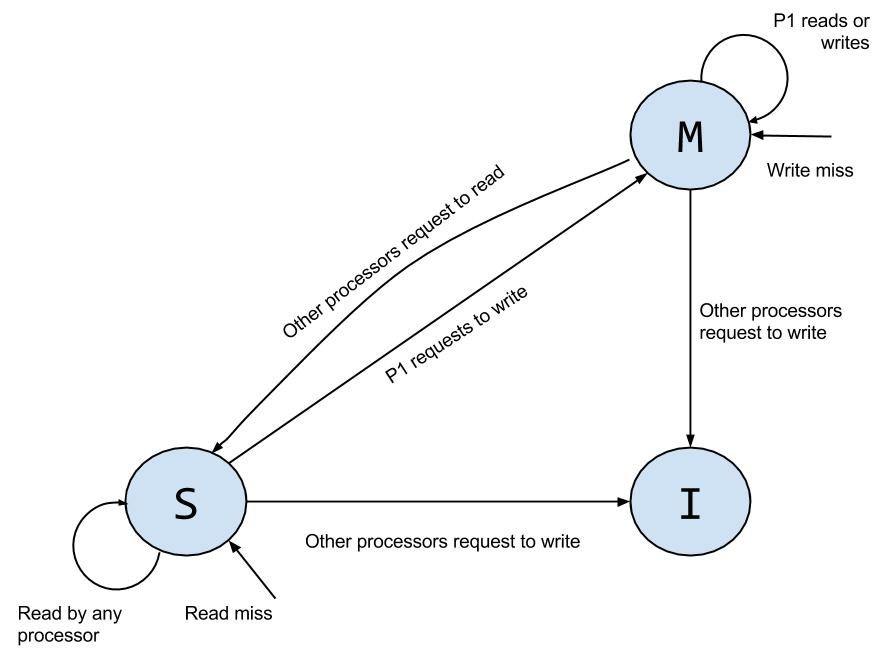
\includegraphics[width=1\textwidth]{img/MSIstatediagram.jpg}
    \caption{MSI State Diagram for processor P1}
    \label{fig:MSIstatediagram}
\end{figure}

In figure \ref{fig:MSIstatediagram}, MSI protocol's state diagram is showed. Cache memory launch with invalid cache block, and when a read miss is comprised,  cache controller will request memory block from memory. Then, the snooping control bus will broadcast the request of read. If there is a modified copy on the bus, it will abort request of memory block from memory. It will evict its line to memory, and change its state to shared state. Then, memory responds source of the request. After the fetching cache block to the source cache it, it sets the state as shared state. If there is a shared stated copies in the system, It does not matter who responds the request. In any case, It will fetch the memory block, and sets the state bits to shared.

When write miss is compromised in invalid state or shared, It will fetch the data as same as read miss cases, but the difference is it will invalidate other case's corresponding block which are shared or modified. Modified stated block must evict blocks properly. At the end, source cache block fetches the block.

Write hit can be compromise in modified state, and read hit can be compromise in shared state.

\subsubsection{MESI - Exclusive}
\begin{figure}[h!]
    \centering
    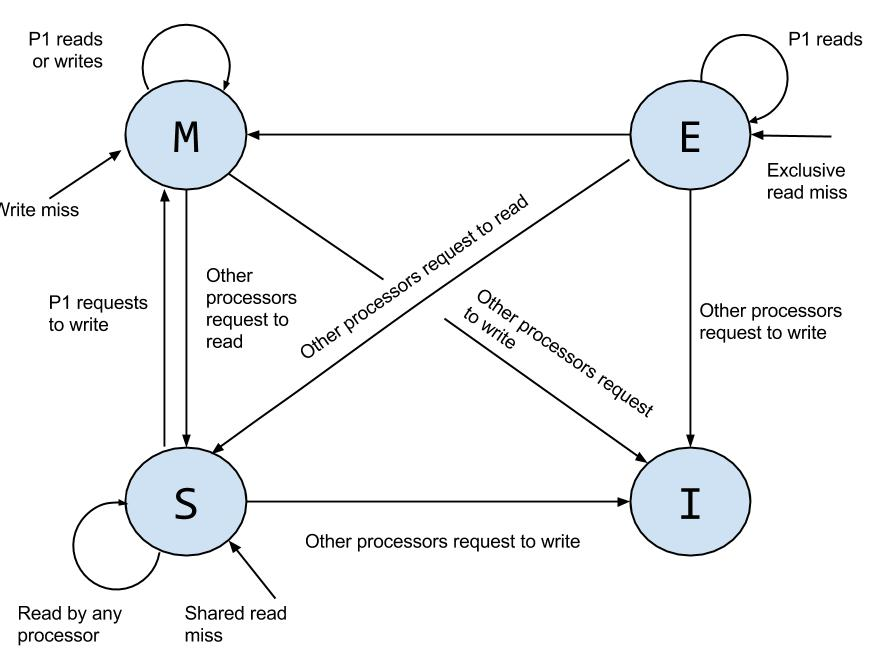
\includegraphics[width=1\textwidth]{img/MESIstatediagram.jpg}
    \caption{MESI State Diagram for processor P1}
    \label{fig:MESIstatediagram}
\end{figure}


The MESI protocol (a.k.a Illinois protocol due to its development at the University of Illinois at Urbana-Champaign) is a widely used cache coherency protocol\cite{papamarcos1984low}. The idea behind the MESI is to use forth state we can use with 2 bits. In order to increase efficiency $exclusive$ state is developed by JH. Patel et. al. in 1984\cite{papamarcos1984low}. As showed in MSI protocol, there is modified, shared and invalid states but also we have exclusive state. This exclusive states also known unmodified exclusive state, if we refer modified state as modified exclusive. This is very similar to the shared state in MSI, and in fact, Shared state is split in two different states. That is because of reducing the communication on the bus and increasing efficiency. In this case, there is exclusive cache blocks which are in read mode and they are unique i.e there is no other cache controller on the system has this cache block. 

\begin{description}
\item[Exclusive] The cache line is only present in current cache memory, and it has not modified yet. It is not a state to provide coherency, but it is state for increasing efficiency of bus bandwidth usage. When a cache line in exclusive state the cache controller can decide the transaction of the line without communicating with other caches. When a cache is requested with load operation, it is loaded in exclusive state, if there is no other cache controller has the cache block.
\end{description}


\begin{table}[position specifier]
\centering
\begin{tabular}{|c|c|c|c|c|}
\hline 
• & Clean/Dirtiy & Write? & Unique? & Silent Transition to \\ 
\hline 
Invalid & Clean & No & No & - \\ 
\hline 
Shared & Clean & No & No & Invalid State \\ 
\hline 
Excursive & Clean & No & Yes & Shared Modified Exclusive States \\ 
\hline 
Modified & Dirty & Yes & Yes & - \\ 
\hline 
\end{tabular} 
\caption{MESI states' properties}
\label{tab:MESItable}
\end{table}

In figure \ref{fig:MESIstatediagram}, state transactions are showed. Bus usage is bottle neck, low performance behaviour in cache coherency. Silent state transactions are transactions in cache controller without communicating with other caches. For example, there is no need to broadcast and occupy bus for invalidating shared state in MSI protocol. If a cache controller is in shared state, the other cache controller can be shared or invalidate in MSI, so there is no dependency in the system transaction from shared to invalidate. Exclusive state is to exploit the salient transactions. When a load request arrive to cache controller from a processor, it request the line from upper level memory controller and other child caches controller. If any child controller send a shared state broadcast message, it load it in shared state. If there is a exclusive cache controller on the bus, it will degrade its state to shared and broadcast it. If there is no other shared state on the bus. It load the cache line in excluded state. Then, in case of store operation from processor, it will transact its state from exclusive to modified. It does not need to broadcast it, because we know it is unique in system. Contrast with modified state, due to be cleanness of the line, it does not need to evict line to upper memory, it can  just invalidate it silently. The weakness of this protocol comparing with MSI, if there is many processor with the corresponding cache line, when it count the copies to test uniqueness, it occupy shared bus more in some cases. If there is n cache controller with corresponding cache line, it will send n broadcast message with this message, however, instead of sending whole line to upper memory it is mostly efficient to send this message.

\subsubsection{MOESI - Owned Exclusive}
\begin{figure}[h!]
    \centering
    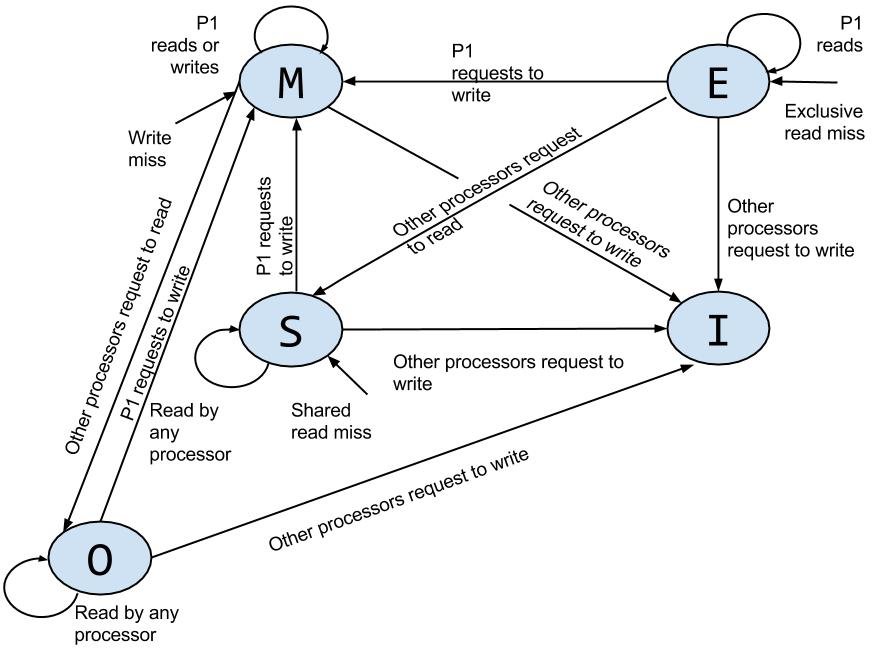
\includegraphics[width=1\textwidth]{img/MOESIstatediagram.jpg}
    \caption{MOESI State Diagram for processor P1}
    \label{fig:MOESIstatediagram}
\end{figure}

\begin{table}[position specifier]
\centering
\begin{tabular}{|c|c|c|c|c|}
\hline 
• & Clean/Dirtiy & Write? & Unique? & Silent Transition to \\ 
\hline 
Invalid & Clean & No & No & - \\ 
\hline 
Shared & Either & No & No & Invalid State \\ 
\hline 
Excursive & Clean & No & Yes & Shared Modified Exclusive States \\ 
\hline 
Owned & Dirty & No & Yes & - \\ 
\hline 
Modified & Dirty & Yes & Yes & Owned \\ 
\hline 
\end{tabular} 
\caption{MEOSI states' properties}
\label{tab:MSItable}
\end{table}

Such processor producers AMD Opteron and Arm Cortex A are using MOESI protocol for cache sharing. In addition to the four states in MESI, a fifth state "Owned" appears here representing data that is both modified and shared. Using MOESI, instead of writing modified data back to main memory, it directly forward the dirty value from cache to cache before being shared, which could save bandwidth and gain much faster access to users to the cache.

\begin{description}
\item[Owned] Owned state is a state if and only if a cache line can transact in it, when a read request message snooped from another processors when the cache line is in modified state. It allows dirty line sharing between caches, and reduce the latency which is arisen due to the communication between memories and processors. The line is read only by all processors, when it is owned state.
\end{description}

In figure \ref{fig:MOESIstatediagram}, state transactions of MOESI protocol are showed. The relationships of states are almost same with MESI, but there is a state which supplants upper level memory with its own cache line. Hence, it is responsible with evicting lines and cleaning state. The cache line may be changed to the Modified state after invalidating all shared copies, or changed to the Shared state by writing the modifications back to main memory. If could increase efficiency sharply, if the line between upper memory and itself is long and bandwidth is limited. Mostly the L1 and L2 caches are located on-the-chip, and memory are located somewhere outside, the buses' bandwidth between in side and outside of chips are game changer. It can be efficient to use a chip as a forwarder in many system. However, in the MOESI protocol, it is not possible to forward the cache line which is not dirty but present on the chip. If there is a shared cache line in a cache, and if any other cache controller request to load the same cache line, it fetches it from memory.


\subsection{Inter-connector Design}
\begin{figure}[h!]
    \centering
    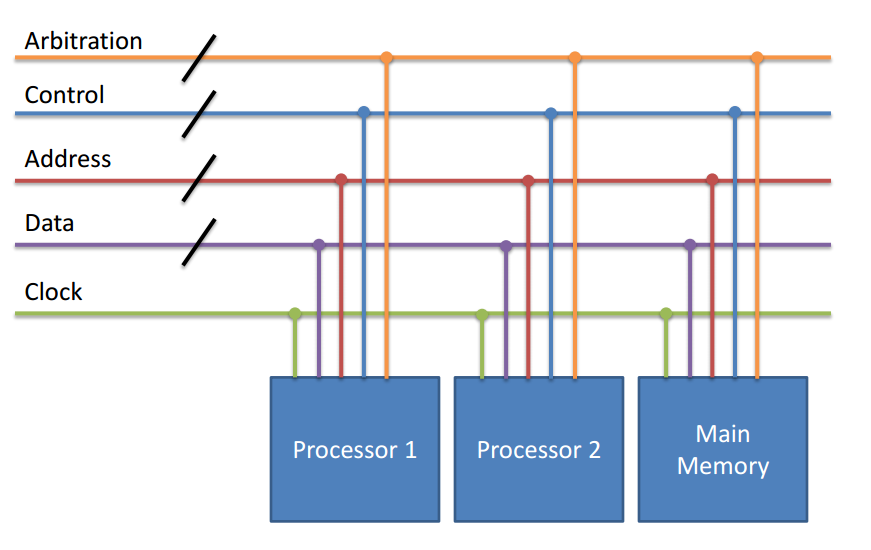
\includegraphics[width=1\textwidth]{img/bus_primatives.png}
    \caption{Primitive Multi-Drop Memory Bus }
    \cite{ComputerArchCoursera}
    \label{fig:bus_primative}
\end{figure}
Computer Bus which is the primitive version of the inter-connection network was designed to transfers data between components inside a computer, or between computers. They are defined to include all computer hardware components and software, included with communication protocols, in order to communicate devices. Devices is generally called as node or end node in taxonomy. However, this definition is quite broad and it covers from today's internet network to cloud computing network and evolved in many aspect to different direction.

In figure \ref{fig:bus_primative}, There is an early multi-drop bus example. Multi-drop bus term is used for a bus line with many element on a line (not a ring), and there is an arbitration mechanism, so it is normal computer buses which is used in interconnection taxonomy. The multi-drop buses includes 5 separated wires which is distinguished by their purpose. Arbitration line decide actually how has right to speak, request. There is a logic devices to determine the arbitration and it is one of the most crucial research area in computer architecture and especially interconnector design\cite{hennessy2012computer}. Control wire is actually determine the purpose of the node. Generally, they are $store$ and $load$ operations. The address wire determine the requested address from corresponding place, in this case there is no cache controller so directly memory. Data wire carries the data which is stored or load, so the communication is synchronous, with consecutively request and reply. Lastly, clock wire provides a fixed, constant frequency to carry values.\cite{hennessy2012computer}

On recent systems the communication mechanism between nodes are quite more complicated comparing with given primitive example. The pace in the development on parallel systems makes correlation and communication between notes chaotic. Systems comprise with many nodes and requires high bandwidths  to overcome and increase their bottleneck. Intercommunication is still the slowest part of mainframe and personal computers. On the other hand, with multi layer memory aspect, communication between nodes and parallel computing gets more and more complicated. It makes every cache controllers a member of interconnector and perhaps  more. Today, there are some coherent interconnector which are also responsible with traffic management (i.e. QoS), barriers between devices and memories, and coherency\cite{armcoherentinterconnector}.

\begin{figure}[h!]
    \centering
    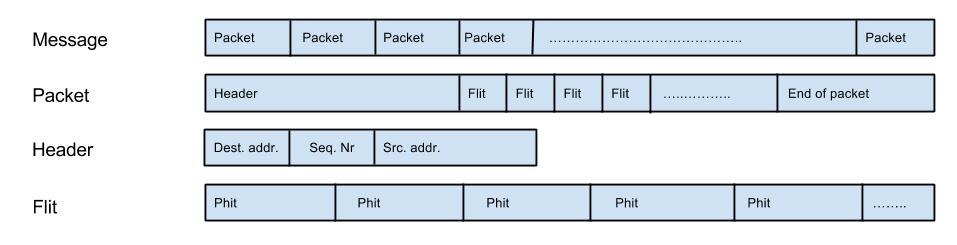
\includegraphics[width=1\textwidth]{img/Message_Anatomy.jpg}
    \caption{An example of interconnector message anatomy }
    \label{fig:message_anatomy}
\end{figure}

There are two main category of computer interconnectors which are host based On-Chip and System/storage area network and remote over LAN and WAN networks inter-connectors. On-Chip networks purpose to mitigate the on-flight latency and chip-crossing wire delay problems related with increased technology scaling and transistor integration. Nevertheless, there is not enough space in a single chip to fill many cores. It is a good design for interconnecting ALU, registers caches, compute tiles, and perhaps several cores and memory. System/storage area networks are the most used interconnection systems between multi-processors, multi-computer, multi-thread systems and memory system interconnection between this cores. Because of physically constrains such as distance and density, it is usual the interconnector between systems and their I/O extensions (e.g DMA chips). LAN and WAN based systems are actually designed to connect enormous number of node together. This kind of networks distributed several locations and interconnecting PCs cluster of computers. Cloud computing is actually one of the good example to show the ability of this species. On of the other advantage of remote interconnectors is that they are generally build on well-known protocols which are tested and acknowledged protocols e.g. Ethernet, GSM, IP, TCP, UDP. All routing issues are tested for many years and solved properly.\cite{hennessy2012computer}.

Modern interconncetors with advance switching and routing mechanism are using message protocols.  In figure \ref{fig:message_anatomy}, an example of simple interconnector message anatomy is shown. Alternatively, the bus anatomy we mention above, the message based protocols are packetized. However, this packetizing process has some overhead as latency\cite{ComputerArchCoursera}. Message anatomy of interconnectors comprises several layers\cite{0122007514}.
\begin{description}
\item[Message]The message is the unit of information which must be transmitted with a propose. If it is about cache coherency, It could be whole line of the cache to provide coherency.
\item[Packet]Packets are the fixed maximum sized  smallest unit of information which include routing information in its header section. It can also include sequence number for flow control protocol. Its size is depending on the arbitration mechanism on the router or switches. It comprises with data flits which actually part of information in message.
\item[Flit]The small unit of link layer is called flit. Flits size are depending on the switching algorithms. In circuit switching flit size are whole packed. They are typically 4 byte to 16 byte.
\item[Phit]It is the unit of the physical layer in the interconnectors design. Its size is depending on the clock cycle of the interconnector. On the primitive bus example, the clock mechanism determine the phit size when it tick. They are around 8 bit to 32 bit.
\end{description}
 In order to characterize interconnector device we will use several feature of networks which are switching mechanism, switching mechanism, routing algorithms, topology, and flow control of networks. These feature are determine depending on application domain and defuse all character of network. Across the designs, performance with latency and bandwidth parameters and queuing theory is the valuable analysis tools to define network and its classification\cite{hennessy2012computer}.

\subsubsection{Switching}
Switching name root originally comes from circuits. It is complex combination of many circuits switch which actually connects conductors together. It determines in interconnection networks how data is allocated for data transmission, i.e. how and when the input channel will be connected to the output channel. Buffer states, channel flow, and surely routing algorithms effects the switching designs as we know so far from computer network design. To sum up, it is actually model how to connect different locations and nodes together.
\begin{description}
\item[Circuit Switching]
\item[Packet Store and Forward Switching]
\item[Packet Cut Through]
\end{description}
\subsubsection{Topology}
\begin{description}
\item[Buses]
\item[Ring]
\item[Fat Tree]
\item[2D Networks: Meshes, Torses]
\item[Multiple Dimensional Networks]
\item[Star]
\item[Omega]
\end{description}
\subsubsection{Routing}
\begin{description}
\item[Deterministic]
\item[Non-Deterministic]
\end{description}
\subsubsection{Flow Control}


%!TEX root = thesis.tex
\chapter{Cache Oriented Obfuscation on the System without Coherence}

In this chapter of the thesis, we proposed a method to design a reliable and efficient obfuscation technique for tightly coupled multi-processing systems by exploiting the feature of cache oriented programming. Besides, we emphasized a number of points to characterize proper attack vector. After we had elaborated our obfuscation methods and its primitives, we discussed what it is and what it is not on pitfalls and fallacies section. Finally, on the implementation section, we drew a picture of possibilities on practical applications. However, this chapter and this thesis does not concern specific and deeper studies on obfuscation and memory protection(TLB, MMU, MPU). They are correlated with our thesis, but it is on the upper layer which is like TCP and IP layers of network. On the whole and in the brief, this chapter gives an isolated workspace for obfuscation techniques.

As we mentioned previous chapters, malware detection tools needs sensors to analysis running code. Regular sensors observes real-time systems with monitoring shared memory, it means a lot for operating systems, because OS, computer architecture and computer conventions assume everything on the memory and ultimate and consistent. With this assumption, dumping memory and analysing snapshots are practically efficient and convenient way of malware monitoring and detecting. There are actually a number of sensor type for real time memory observation: external monitors, internal monitors, and exotically virtual monitoring. External monitors in contrast with internal monitors are the systems which is comprised with external hardware devices and its software component. They could be implemented on external PCI or GPU devices, FPGA co-processor or on-board chip\cite{Christos2013}. They are efficient because they are pre-installed, omnipresent systems which does not require OS and other middleware platform which constrains their limits. Also They are efficient because they are the hardwares which can be designed with the purpose. However, they are expensive to implement comparing with internal monitors. Internal monitors are using regular devices on the computer architecture such as CPU, and they are working under the operating systems' kernel, which could be easy to deceive \cite{Adnan2011}, \cite{rutkowska2006rootkits}. Our methods is actually not depending on the monitoring type, since it is related with where they are monitoring.

Tightly coupled multi-processing systems have many processor with their own caches and one shared memory\cite{Jim2007}. Cache memories are not developed with same purpose of memories, but are developed for performance reason which we discussed in background studies. If we exploit them and design our program properly, cache memories could be used as another layer of memories, and on the monitoring side, even if it perfectly scan and detect memories, cache memories are still out of the box.

The required systems for our technique in this chapter is tightly coupled multi-processing systems without cache coherence interconnector. Also, we need simple Harvard computer architecture instead of Von Neumann. Incoherent systems are surprisingly popular because of the implementation errors i.e. Samsung's mainstream CPU Exynos 5410 which sold millions, and also due to costs. Many hardware designers also believe programming with shared memory is not appropriate way and platforms such as Android already using message based communication on multi-threaded application, and  they implement clustered processors which limits programs instead of implementing expensive coherency interconnector. Yet they do not consider security approaches.
    \begin{figure}[h!]
        \centering
        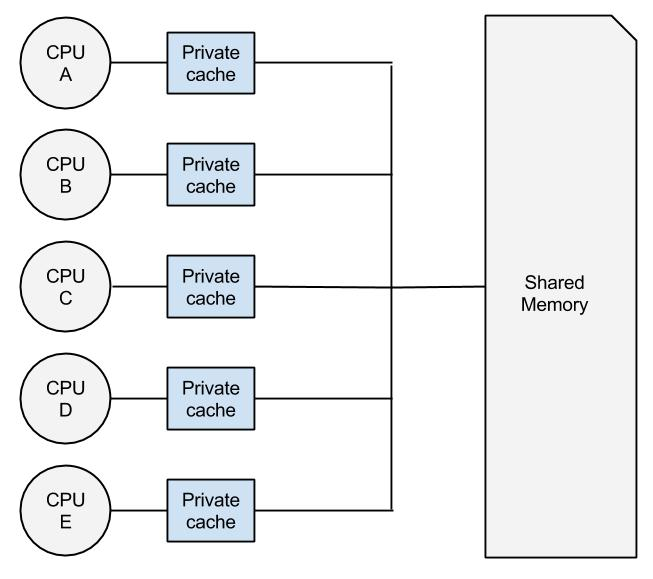
\includegraphics[width=1\textwidth]{img/Tightly Coupled Multi-Processing Systems.jpg}
        \caption{An Example of Tightly Coupled Multi-Processing Systems}
        \label{fig:tightlycoupled}
    \end{figure}
	

	\section{Exploiting Tightly Coupled Multi-Processing Systems}
	    \begin{figure}[h!]
	        \centering
	        \includegraphics[width=1\textwidth]{img/attack vector.jpg}
	        \caption{Attack vector flow chart}
	        \label{fig:atackvector}
	    \end{figure}
	    \subsection{Reconnaissance and Design}
	    \subsection{Setting system up and Loading Cache Memory}
	    \begin{lstlisting}
	mov r2, 0x012345 #address
	mov r3, 0x013456 #end of gadget
	mov r4, 0 #counter
fetch: 	addi r2, r4 # add size of word to address
	mov r1, [r2] #Load address from memory
	cmp r2,r3 # compare r2 and r3
	jl fetch
\end{lstlisting}

	    \subsection{Obfuscating Running and Deobfuscating gadget}
	    \subsection{Regeneration}
	\section{Pitfalls and Fallacies}
			Coherency Mechanism
			Harvard Arch
			Caches are not memory
			Context switching


%!TEX root = thesis.tex
\chapter{Probabilistic Timing Attack against to Snoopy Cache Coherency}
In this chapter of the thesis, we proposed a probabilistic attack to increase evasion probability of malware against to snoopy cache coherence protocol on tightly coupled systems with write back cache policy. We briefly explained the issue we can encounter during implementation of the cache oriented obfuscation method with the snoopy coherent systems. The snoopy cache coherency protocol's internals have already been mentioned in background studies chapter; however, we assumed through whole section that all coherence operations are atomic, and contention between processes are not subject. Yet, They are not close to be atomic; and moreover, the latency is sometimes enough long to process and to complete whole gadget or whole malware. In order to exploit this contention, we methodized a probabilistic race condition attack. 

As a brief and in other words, instead of giving an absolute obfuscation, we proposed a method which probably obfuscates malware, and this probability depends on the systems design and gadgets' processing overhead. On the other hand, this value gives us a quantitative rate, but if our concern is signature based detection methods, signatures' value can be measured with qualitative approaches rather than quantitative ones, e.g. some signature like port number or IP address are treasury.  Yet, the quantity of signature is certainly another value to measure efficiency, especially when we relate binary codes and signature detection.
\todo[inline]{Add more details about how lazy they are}

\section{The Issue}
Cache coherency is a term and discipline arisen from the incoherent states of caches due to parallel computing. It does not need multi processor environment. For incidence, sometimes, DMA devices can be enough to emerge it. In tightly coupled systems, because of the usage of caches to increase performance, it is highly possible to falling into an incoherency state. We also mentioned much more details in background studies chapter. in this chapter, the term of "stale data" is used to describe globally\footnote{In local frame, it concerns the relationship between the CPU and cache values rather than between caches. } the data which is not reflected for most current or synchronized value in the system(included with other caches and memories). In order to synchronize stale data and provide coherency between caches, cache coherency protocols and policies are used between caches. As we mentioned, most of  protocols and policies need networks between each other and logical operator per cache controller. There are many methods to provide coherency between caches and one of the most known and capable one is snoop mechanism. 

Snoopy cache coherency mechanisms provide synchronization with a bus watch mechanism in the system bus. These mechanisms imply that cache must first request the data from any other caches, before it request from the memory. The implementation of the snoop mechanism is vice versa, but works as well, as same.Cache generally watches the bus and record activities, arise exception in case of coherency problem(when it is likely to fall incoherent states).\cite{Jim2007} There is generally an interconnector to organize snoopy cache protocols, and filter useless communication. 

Moreover, the nature of the cache organization which we use commonly is lazy. The mean of lazy is they do not update the modified block and values until they evict and replace it with other cache block. The reason why they are lazy is obvious, the efficiency optimisations. If they write every modification directly memory as well as cache\footnote{It is salso  mentioned in background studies as write through policy}, it will consume most of the available bandwidth. The main essence how we keep our data in a cache as like as private memory is arisen from this laziness, because we anticipate and controls the cache line evictions and replacements. However, we cannot simply say write-through caches are perfectly coherent because of the reasons explained in Chapter 3. For example, $CacheA$ read address $x$, and then, $CacheB$ read address $x$. If $CacheA$ write address $x$ with Write-Thought policy, the value in $CacheB$ is still stale.

With perfect coherent caches, we can not exploit private caches to use as private memory (see also. NUMA); hence, we can't evade anything from one CPU to another as we did in the previous chapter. Namely, there is no difference between disk to memory and disk to cache obfuscation. Even though the highest workspace which you deobfuscate your code is cache, cache are synchronizing each other. This coherence gives ability to anti-malware scanning other caches and detecting signature.
\section{Solution}
	Let's assume we have a tightly coupled multi processor test bed system, and it has one CPU reserved to scan memory for malware detection, and another CPU is occupied by malware itself. Their caches are snoopy coherent with an interconnection network.  They could use any of protocols which we mentioned in background studies e.g. MOESI, MESI, MSI. Let's also assume that the malware which present in the second CPU's cache is designed as we defined in previous chapter. It has prewarmed cache as we described and started to deobfuscate and run the code. The presumption is the $CACHE 2$`s cache blocks is accessible by $CPU1$ as well as any other CPUs. However, the access and synchronization of any stale data is not that simple. It is presumed as atomic, but it is not, and worst of all, tightly coupled systems are heterogeneous with cache coherency, because the distance to memories are not equal and systems are not homogeneous. This heterogeneousness comes with different access times to the memories. Especially MOESI protocol is much more heterogeneous because it works as semi-NUMA(Non uniform Memory Architecture) type cache i.e. a modified cache block can be moved around various caches without updating main memory. Secondly, cache controllers rule are not really elastic. When an address is touched by a CPU, it fetches whole block in order to exploit spacial locality and increase performance\footnote{Sometimes they wait for feeding CPU until fetch it all, sometimes feed CPU as soon as possible depending on algorithm.}. We actually exploited throughout whole chapter two weaknesses which are horizontal directional cache fetching attribute and synchronization latency and heterogeneous access time of snoopy caches.
\subsection{Horizontal Directional Cache Fetching}
In computer architecture conventions, we arrange instructions into memory space, incrementally, and then, we can prefetch them before they run. Also, we are tent to use the space around we recently accessed. It is called spacial locality and we mentioned about it more deeply in background studies. For this reason, we cache mechanisms works horizontally. It fetches a particular size of memory in the same time, and put it a cache block. Besides, cache blocks are the smallest addressable memory spaces; therefore, it makes caches more simpler, faster\footnote{After an amount of memory, it could decrease performance.\cite{ComputerArchCoursera} }and cheaper. Accordingly, Fetching and eviction operations are handled as line-based namely horizontally. 
	\begin{figure}[h!]
	    \centering
	    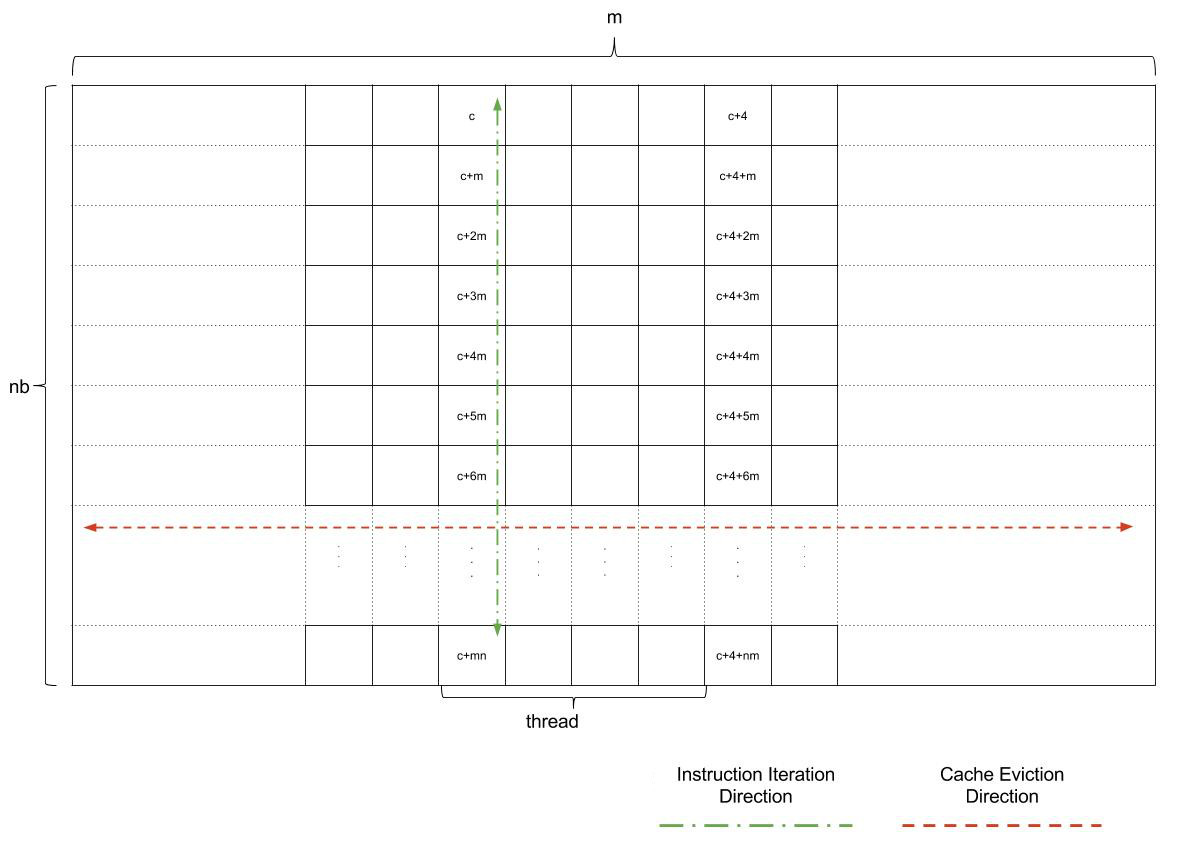
\includegraphics[width=1\textwidth]{img/vertical_instruction_iteration.jpg}
	    \caption{Directional Exploitation}
	    \label{fig:veriticaldirection}
	\end{figure}
In figure \ref{fig:veriticaldirection}, we showed data fetching direction and its contrast with our instruction iteration direction approach. As we mentioned many times, but in order to emphases it one more time, instruction sequence normally increments one by one. Yet, in our approach it iterate as in equation 5.1. $m$ is the cache block size, and $n$ is the number of cache block line in the whole cache. $nb$ is number of line which is allocated to body of our gadget as mentioned in previous chapter, so this figure is a frame of cache in which obfuscated part of our malware allocated. Let's say $c$ is the initialization point of our malware. When $i$ is the number of instruction on the queue, $I(i)$ gives us the location of instruction in the memory; thereby, in the cache. 
\begin{equation}
	I(i)=m*(i\bmod{(nb)})+((\left \lfloor i/nb \right \rfloor*thread)+c)\bmod{m}\\ 
\end{equation}
$thread$ value in the cache is step number between the vertical blocks. In order to generate a function which onto(bijective) the cache frame, equation 5.2 must be provided, because after it overflow mod function, it will uses just the one next block which previously used and go on until end. It is obvious that $tread$ should be smaller than $m$, yet it is already in mod and $i$ must be smaller than total size. 
\begin{equation}
	\forall\: m\bmod thread = 1\ :\  I()\ is\ bijective\ function
\end{equation}
Yet, Why do we iterate institution sequence  vertically? Indeed, we assumed that anti-malware scans horizontally from $CPU1$ above, because it is faster. For example, our code starts from $c$ and our second instruction in $c+m$, with purpose of scanning from $CPU1$ in this order, it should  fetch first the line of $c$ into $Cache2$, and then, it should fetches the line of $c+m$, and so forth. In the perfect world, with atomic instruction to fetches whole cache line and without latency, it could be race condition free approach, but in real systems, it is not. We will combine this attack with latency problem in the next sections.
\subsection{Synchronization Latency of Snoopy Caches}
One of the famous myth on the computer science and design is that tightly coupled parallel architectures are mostly considered as symmetric systems, but if we look more closer, the caches usage and moreover cache usage with coherency protocols and network makes them quite asymmetric and preforce them to be heterogeneous. Processors could have same properties and be arranged in symmetrical, but if they can't give same throughput in an time interval, we can't call them homogeneous\footnote{In order to prevent this, there are systems which avoid to use caches, when they are sharing data. Because of the symmetry of cache processor relationship, they keeps their symmetric design themselves.}. 


\subsubsection{Latency Calculation}
	\begin{figure}[h!]
	    \centering
	    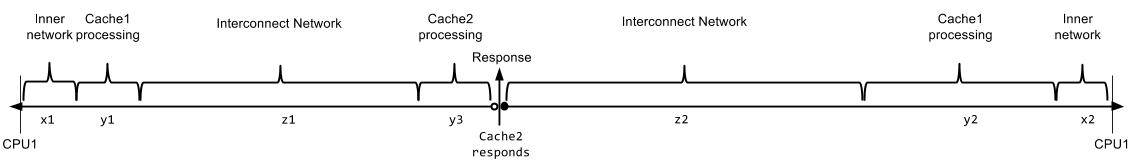
\includegraphics[width=1.1\textwidth]{img/timing_diagram.jpg}
	    \caption{The Time Line of the Fetching Cache Line which is Used by Another Cache}
	    \label{fig:timeline}
	\end{figure}
In figure \ref{fig:timeline}, we showed a representational illustration of cache line requesting process which is used in another cache, and labelled latency types with $x$ for inner network latency, $y$ for cache processing latency, $z$ for overall interconnection latency. As seen in figure \ref{fig:timeline}, the throughout latency for synchronization process with another cache is showed in equation 5.3. However, the latency of direct reaching to the cache is showed in equation 5.4 which is obviously shorter\footnote{This formulas are valid for the simple systems showed in figure \ref{fig:tightlycoupled}}. 
\begin{equation}
L_{s}=x_{1} + y_{1} + z_{1} + y_{3} + z_{2} + y_{2} + x_{2}
\end{equation}

\begin{equation}
L_{d}=x_{1} + y_{d} + x_{2}
\end{equation}
All this latency variables is depending on many different factors which we can calculate them in theory, but which is difficult to estimate in practice. $x$ variables are the latencies between CPU and cache. It is tent to be really short, because $L1$ cache and CPU should be designed so close. Mostly $x_{1} = x_{2}$, yet it is not certain. The reason is write buffer and pipelined CPU makes it case depended. Generally, most of the latency comes from the queue of cache which also related to writers block and pipelined architecture as we mentioned in background studies. $y$ variables are cache's logical response latencies. As we mentioned, It depends on cache size, associativity, line size and logical operations complexity. In this example, we have one layer cache, but most systems use multi layer caches. For each layer, it adds more overhead. In brief, caches are as fast as how simple they are.\footnote{Their design affect performance a lot, but they are mostly SDRAM instead of DRAM or switch based registers} However, there is no doubt that most important and game changer latency is $z$ namely, interconnection network latency. 
	\begin{figure}[h!]
	    \centering
	    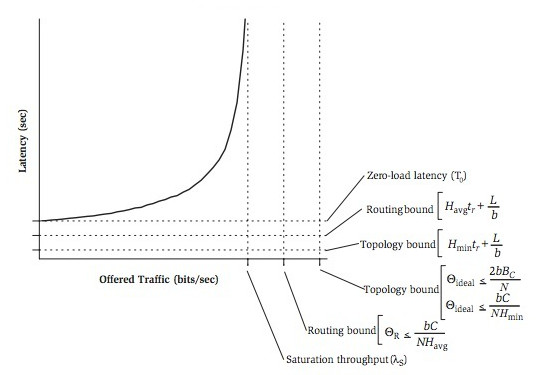
\includegraphics[width=1.1\textwidth]{img/latency_graph.jpg}
	    \caption{Interconnector Latency Versus Offered Traffic \cite{0122007514}}
	    \label{fig:latencyvsofferedtraffic}
	\end{figure}
 Mostly, lack of bandwidth is considered as the only reason of network latency, whereas there are many other factor and problems. Nevertheless, it is one of the most important source of latency. Bandwidth is the rate of the data can transmitted from point $a$ to point $b$ in a given time, but originally, it was the number of wire in width of buses. This definition ignores the clock speed contrast with current definition because the speed of wire is related with speed of light and resistance of the wire, but instead, the things which limit it is the performance of source and receiver. The bandwidth could be formulated as $ b = n * f$ where n is width of the channel and f is clock speed. Surprisingly, if our message is smaller than channel width, bandwidth can not effect latency because if we have 100 bit bandwidth, then it carries 20 and 100 bit in the same time. Notable the interconnection networks' costs are routing, serialization/deserialization, link traversal latencies\cite{0122007514}. We already have mentioned about their details; still, it is good to shortly recall that serialization and deserialization are processes to converting messages to given channel bandwidth and could be shown as $ sd = L / b $ where $L$ is length of message and $b$ is bandwidth. Therefore, overall latency can be measured with formula 5.5.
\begin{equation}
T_{0}=\sum_{k=1}^{minr}tr_{k}+\sum_{k}^{minc}D_{k}/v_{k}+L/b
\end{equation}
In this equation, $minr$ and $minc$ denote the minimum number of router and channel between point $a$ and $b$. $tr$ denotes time consumed during routing process, while $D/v$ denotes distance divided by velocity. The easy way to calculate $T_{0}$ for each flit is $T_{0} = T_{head} + L/b$ because $\sum_{k=1}^{minr}tr_{k}+\sum_{k}^{minc}D_{k}/v_{k}$ is calculated one and only one time in pipelined networks as have been mentioned. If it is not pipelined, the latency could be measured by formula 5.6 or if it was store and forward flow control instead of cut-through as shown in equation 5.5, the latency could be measured by formula 5.6 (see more details \cite{0122007514}). 
\begin{equation}
T_{0}=(\sum_{k=1}^{minr}tr_{k}+\sum_{k}^{minc}D_{k}/v_{k})*L/b
\end{equation}
\begin{equation}
T_{0}=(\sum_{k=1}^{minr}tr_{k}+\sum_{k}^{minc}D_{k}/v_{k})+(\sum_{k=1}^{minr}*L/b)
\end{equation}
However, $T_{0}$ is not a general latency function, and it is very special status of networks which is also called zero-load latency.  Zero-load latency is the lowest bound of the latency where there is no contention between packets. In figure \ref{fig:latencyvsofferedtraffic}, a generic latency vs offered traffic curve is showed. Although they are the most accurate way to measure and determine ultimate performance, and we are using discrete event simulation to draw them. Theoretic latency bounds, which are topological and routing, and their corresponding throughputs are showed in figure. In formula 5.4, 5.5 and 5.6, zero latency values are all shown with minimum routing hops which means topology bounded zero latency, but actual zero-load latency, $T_{0}$ in figure, incorporates the constraints of topology along with actual performance, routing, flow control and line traversal latency\cite{0122007514}. As have seen obviously, if you increase the contention between packets through increasing offered traffic, the latency grows about exponentially. It is one of the most important factor support our proposes and encourage us to implement because of the fact that roughly loading memory and storing back to the hard disk\footnote{It is basically dumping memory} produce remarkable traffic which can lead considerable latency.

\subsubsection*{Simulation Result}
	\begin{figure}[h!]
	    \centering
	    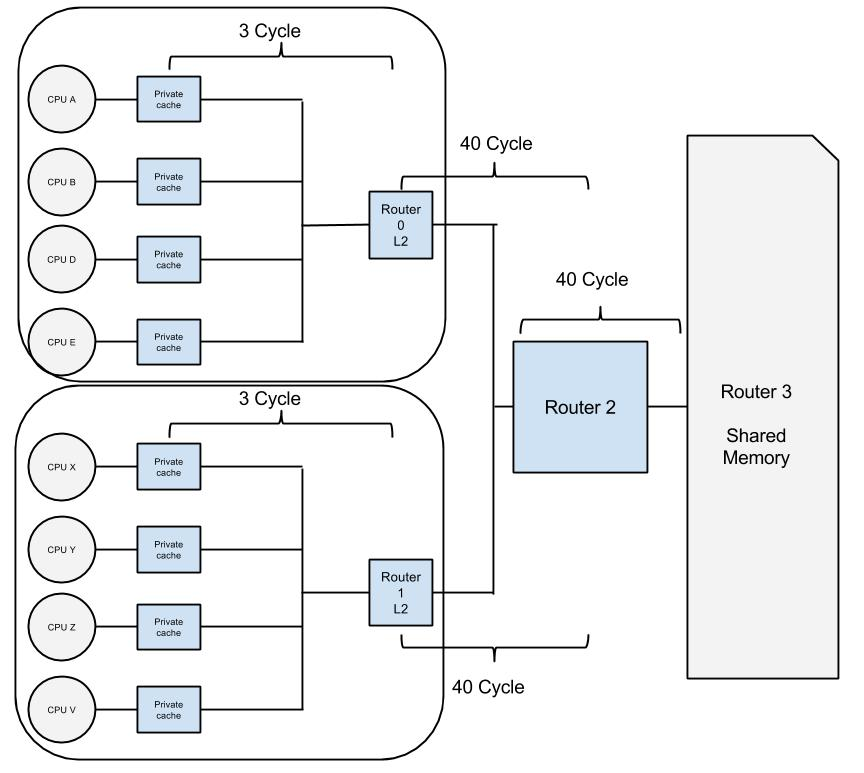
\includegraphics[width=0.8\textwidth]{img/simulation.jpg}
	    \caption{Our Simulation Topology\cite{0122007514}}
	    \label{fig:simulation}
	\end{figure}
An accurate simulation is definitely one of the most important tools for analyzing interconnection networks and exploring design tradeoffs. The reason why we are using simulations instead of real systems is a bit similar with theoretic physic. There are many noises on information we gathered from real systems and they are extremely expensive and difficult to implement. Even one of the most acknowledged books about interconnection network, which is called "Principles and Practices of Interconnection Networks" repeatedly emphasizes that designer's intuition is the most important factor to design better performance on interconnection networks\cite{0122007514}. This book has a simulation tool freely available at http://cva.standford.edu/\cite{jiang2013detailed}. Even though, every processor company invests their years and efforts to design better simulator, this tool is quite simple and totally free licensed. However, it is not designed for coherency purpose, so its model designed in flit level and includes many topologies and routing algorithms. Indeed, it can give us some important cues and ideas. 

We designed it with an example topology which we use in multiprocessing systems. It is the inheritor topology of Fat tree. In figure \ref{fig:simulation}, the topology is shown which has two processors, 3 routers\footnote{Though we said 3 routers, we used in figure and topology design file 4 router. That is due to lack of simulation tools. We tried to give a latency between router 3 and shared memory} and shared memory. This designed is influenced by one of the most known ARM chips Samsung EXYNOS 5420. This latency values are rounded numbers, but they are close values which we obtained the concerned chip\footnote{we used CPU-Z program to measure cache latencies.}. One way channel length is about 3 cycles from L1 cache controller to L2 cache controller, 40 cycles from L2 cache controller to L4 cache controller. This contrast could be because of the difference between in-chip out-chip communication and also the complexity of caches internal operation. We assumed the routing delay is about 2 cycles, even though it could be a bit more. We used 1 cycle credit delay for flow control.

The injection rate of simulation is the number of packets which it injects every cycle time. The book claims average rate is 0.15, but we consider that it is enormously high for our experiment. As we have said, injection rates could be really high during memory dumping; however, it could be decreased, if scanner avoids bad programming practice and exploit cache performance feature, it could be around one store and one load operation request  for each cache block from upper layer cache. If we take this into consideration, we assumed the injection rate 2 and 4 for each 100 cycles. It is also good to assume it lower for any cases. 

One of the other important value about our experiment is the character of our generated traffic. We used a uniform traffic generator which means every nodes talk with each other. However, it is not actually appropriate for our attack. In our example, scanner $CPUA$ talks a lot, and other CPUs talks nominal, but $CPUX$ attacker CPU does not load or store, after it initializes. We can implement our own traffic generator for this simulator in the future. This simulator is also highly adaptive and extensible with plugins.

In implementation of our topology, we decided to design two different modes to emphasize contention over network, which are small topology and crowed topology. In the small topology experiment, we assumed there are just two active nodes, three active routers and one shared memory in the network and they are the ones which connected to $CPUA$ and $CPUX$. In this example, latency is mostly based on distance and pure logical complexity, rather than contention of routing or bandwidth. In the second experiment, we designed the crowded topology which has four nodes connected to $router0$ four nodes connected to $router1$, and they are all connected to $router2$, and also we presumed there are two "slave nodes" which might be DMA devices and one GPU connected to $router2$.

\begin{table}[h]
\begin{tabular}{|l|c|c|c|c|}
	\hline
                  & \begin{tabular}[c]{@{}c@{}}Packet latency\\ Min/Avg/Max\end{tabular} & \begin{tabular}[c]{@{}c@{}}Network latency\\ Min/Avg/Max\end{tabular} & \begin{tabular}[c]{@{}c@{}}Flit latency\\ Min/Avg/Max\end{tabular} & Hops Avarage \\ \hline
Crowded 2\%            & 164/68045/171627                                                     & 13/417/1487                                                           & 13/353/1487                                                        & 2.04442      \\ \hline
Small 2\%            & 8/72/216                                                             & 8/72/216                                                              & 8/72/216                                                           & 2.30611      \\ \hline
Crowded 4\%            & 15698/178598/458108                                                  & 13/410/1736                                                           & 13/353/1736                                                        & 2.04591      \\ \hline
Small 4\%            & 8/322/1273                                                           & 8/129/376                                                             & 8/129/376                                                          & 2.33081    \\ \hline
\end{tabular}
\caption{Simulation Results Comparison}
\label{table:simulation}
\end{table}

The result of the simulation is added in appendix B, and briefly showed in table \ref{table:simulation}. We made four experiment with two different topology and two different injection rate as have been mentioned. For more details, you can check appendix B. We present in this table three different kind of latencies. Flit latency is a simple latency time required from the beginning of flit till end. Latency of a packet is measured from the time its head flit is generated by the source to the time its tail flit is consumed by the destination. Obviously, flit latency is the delay time for transferring a flit from one node to next node which routers applied as node in this case. The contrast with network latency and flit latency is tricky. Network latency is flit latency plus extra serialization and routing costs. Hops average is the average number of hops every flits traversed (except source hop) during experiment. It could give an idea about distribution of message. As you can see, the average hop number is lower on crowed topology because nodes under the same router can talk with each other i.e. $CPUA$ can send a message to $CPUB$ as well as $CPUX$ does $CPUY$. The value which we concern is packet latency, because packets are smallest meaningful communication object. To provide coherency, cache controllers communicate with packets between each other. 

As you can see, on an typical crowded network, average latency varies around $68000$ cycle to $178000$ cycles. If we assume clock cycle is around $1 GHZ$, $100000$ cycle is about 0.1 second absolute time. On the other hand, it is around 72 to 322 on small sized topology. However, if we concern the communication between $CPUA$ and $CPUX$ it is at least $40$ cycles + $40$ cycles + (3 * routing costs) + $3$ cycles + $3$ cycles = $92 cycles$ because of the distance. It means that the latencies we need to concern is above average and close to upper bound because $CPUA$ and $CPUX$ is one of the farthest couple.

It is hard to point an exact average latency value for any system, even if we are exactly sure about target system. The contention is the most important factor for latency. In order to increase the chance of our attack we could use noise production methods from other nodes, but because of its character and highly detectability, it is not recommended, still the scanning and storing processes produces enough latency due to high dependency of memory load store operation. 

\subsection{Overall Explanation of the Timing Attack}
\begin{figure}[h!]
    \centering
    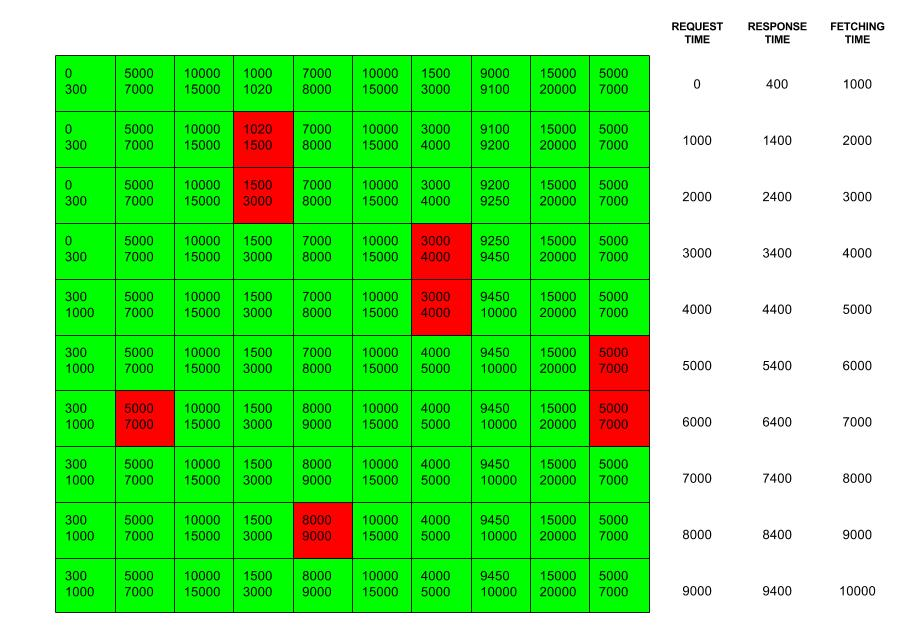
\includegraphics[width=1\textwidth]{img/overall_timing_attack.jpg}
    \caption{The illustration of cache and time Interaction is showed with leaked portion of obfuscated data}
    \label{fig:overall}
	\end{figure}
	Let's presume again we have a malware which is designed as we have proposed in chapter 4 and we have the same system which we have designed in figure \ref{fig:simulation}. Then, the malicious malware is loaded from non-volatile memory e.g. hard-disk to memory obfuscated and it loaded to the cache which belongs $CPUX$. It arranged the structure of cache as have been mentioned in previous proposal. It have been designed as same as it was so far. The point in this situation is we have a memory scanner and dumper application which works in another cache (in this example it is the cache belongs $CPUA$.), and we assume $CPUA$ has coherent cache with $cache x$. This coherency can be provided with snoopy cache coherency through one of the protocols of MEOSI, MESI, MSI. After malware loads the obfuscated code from the memory to the cache, it is allocated as shared state in MSI or exclusive state in MOESI and MESI. It is good to know that it is not going to transmit to modified or owned state until it deobfuscate it. The things which we don't want to share is plain data, and lets call this action as leakage. When we de obfuscate the code, its block in the cache transmits to modified state. Then, if an scanner cpu, $CPUA$, request the block line which we deobfuscate, the long adventure of synchronization starts.

	Our stepped control flow approach has already be proposed as a solution for coherency because instead of whole cache block line leakage, it will lose one step during even theoretical atomic snapshot, and strongly probably it is not going to be meaningful to be signature; however, this stepped approach is not completely good because of its complexity and the effect of that complexity over stub which increase the chance of detectability. The attack we have proposed in this chapter is starting with arranging the steps(more flexible steps, more likely to be smaller gadgets) to the cache vertically as shown in figure \cite{veriticaldirection}, with given formulas 5.3, 5.4. 

	The example which we illustrated is shown in figure \ref{fig:overall}. The time zero on this example is representing the time of the first moment which actually scanner reach the memory location of malware, while the malware's process is flowing. We have another latency assumption here the latency of $x1+y1+z1+y3$ in figure \ref{fig:timeline} is equal to 400 cycle time and $z2+zy2+x3$ is equals to 600 cycle time. The second one is longer because first one which request the cache line is a packet with a header flit, and tail flit. On the other hand response packet comes with whole cache line\footnote{the experiments we made with Booksim 2.0 showed this values as nominal network latency for the topology we designed}. The response time, which we showed in figure \ref{fig:overall} and mentioned in figure \ref{fig:timeline}, is the moment, after it received load request from $CPUA$ and responded it with the cache line. In this moment, cache line is not in modified state, since it is transmitted to the owned or shared state. The interesting point is here that if $CPUX$ manages to write back obfuscated value in place of plain value, then the cache controller of can synchronize this value before scanner detect or store it\footnote{this synchronization could be quite fast with MOESI protocol because $cacheX$ probably allocated it with owned state}. 

	If you look at figure \ref{fig:overall} again, the time intervals which they are deobfuscated and plain showed in the boxes. These intervals are the vulnerable moments for leakage. However, they are ordered vertically, so they can not be fetched in the some time from another cache. The leaked boxes are showed also in the figure. They are the cache block whose line is synchronized, when they are deobfuscated. For example; the first red block on the second line is sent to $cacheA$ at 1400 cycle time, and it was using from 1020 till 1500 cycle time. Therefore it is leaked. However, there are just 8 boxes over 100 boxes overall.

\subsubsection{Overall Obfuscation Rate Calculation}
In order to calculate overall obfuscation rate, we can use formula below. 

\begin{equation}
	\frac{totalblock-leakedblock}{totalblock}
\end{equation}

However, it gives you an quantitative rate which does not represent whether it is evasion or not. Evasion is more depended on qualitative approaches rather than the percent age of obfuscated block because the signature which we uses for detection is generally some strings such as IP addresses or domain names. Of course, the instruction structure is important especially with control flow graph detection, still majority is string searching. The leakage from these strings could be fatal for evasion, even though their size are relatively smaller. Nevertheless, it can imply a general perception about how successful obfuscation we have. It is not going to be same for even particular system and latency, but the mean of many attempts is reliable. So lets formulate it for better accuracy like below:
\begin{equation}
	\frac{\sum_{1}^{n}\frac{totalblock-leaked}{totalblock}}{n}
\end{equation}

In order to increase obfuscation complexity, the exotic kind of settlement structure can be proposed as vertical settlement have been proposed e.g. crosswise, curved so forth. Complexity is not good security practice, but can be useful and necessary for obfuscation. This attack, which we proposed  throughout chapter, will absolutely work with some degree of evasion, but the thing which determines its success is latency of interconnetion network and so, their designs and their logical complexity.

\section{Pitfalls, Limitations and Fallacies}
Even though our methods are novel and theoretically possible, we skip many details in this chapter. For example, the deadlock and live locks in interconnection networks are one of the most common problems. In order to break coherency, they could be useful to exploit, however, it is another attack and vast area. However, it is theoretical likely to appear, if there are to node which share same resource in the same time. 

We also did not mention so much about coherency protocols in this chapter, but they could be useful or problematic depending on case. For example, while you are running around malware cache, if there is another CPU who try to scan you cache, it cat not simply modify cache. Instead, it will demand right of modify for cache line, then other cache controller invalidate the line and then respond to the cache which want to write. It require a lot of time\footnote{As we mentioned in background studies chapter it is a lot more flexible}, and it is the thing can be resulted with deadlock. In addition, this latency could be useful to detect a process of detection. Namely, if there is a difference between write latency, it could be signature of coherence request, but it can't be useful for prevention against scanning.

In the example we showed in figure \ref{fig:overall}, the malware's processing flow spread around the whole cache equivalently, but the most of common processing flow of regular malware are normally comprised with long period of time delay algorithms or watch dog instructions. In these cases, the only thing scanner can obtain is useless instruction which can not be useful to identify malware.

We did not try to calculate process overhead in this chapter, but it is all about contention and race between latency and process overhead. The reason why we did not is that In modern computer architecture, it is quite difficult to calculate it because of the pipelined and out-of-ordered processors. They can process many instruction in the same time concurrently and simultaneously. We should be aware of this, when we design malware. Arranging different kind of instructions sequentially makes it more faster and concurrent, even if we have one core. You can see more details of this architecture in figure \ref{fig:blockdiagram}\footnote{Computer architecture: The quantitative approach book is the one of the best resource about them\cite{ComputerArchCoursera}}.

Memory management and protection units are also the subjects which we never mention in this chapter, yet they are making this attack a bit more possible because they produce extra traffic and extra logical complexity and worst of all, they increase traffic exponentially, however, today, there are interconnector chips for multi processing system which handle memory management itself i.e. Arm CCI 400, 500.
%!TEX root = thesis.tex
\chapter{Implementation on Harvard Computer Architecture}
In this chapter of the thesis, we proposed a method to solve implementation issues on Harvard architecture or equivalent designs. We explained the Harvard computer architecture internals and connect semantic relation between our cache oriented obfuscation technique in order to emphasize details. After we had elaborated the issue with Harvard model, we proposed a theoretical novel solution. Then, we showed several implementation techniques with FORTH programming language. Lastly, we discussed the pitfalls and fallacies in the final section.

\section{The Issue}
	Harvard model is a one of the most famous computer architecture model which contrast with other models with its memory pathway implementation. Basically, there are two acknowledged computer architecture model which are Harvard and Von Neumann architectures. Von Neumann model is an of the basic definition of computer architecture which is first designed in 1945 by Von Neumann\cite{von1993first}.  He describe one of the earliest electronic and digital computation machine and divide processing units in several subdivision consisting of an arithmetic logic unit and processor registers, a control unit containing an instruction register and program counter, a memory to store both data and instructions, external mass storage, and input and output mechanisms. Harvard architecture is an evolved version of Von Neumann Model rather than being complete new approach. Harvard architecture first appeared with "Harvard Mark I" relay based computer, because it was a primitive modern computer which stored instructions on punched tape (24 bits wide) and data in electro-mechanical counters, whereas it's usage purpose is totally different.

	At first glance, having separated memories could sound absurd i.e. Flexibility of one unified memory increases the programmer's ability, but if you look at deeper, there are many reasons to use separated memories. They are increasing performance, especially on pipelined processors, provide wider bandwidth and natural routing mechanisms to spread bandwidth equally, and reduce power consumptions. However, there are also middle ways between these two architectures. If Harvard model implemented on cache layer, and unified memory is preferred as a main memory, it is called Modified Harvard architecture. Most modern computers that are documented as Harvard architecture are, in fact, Modified Harvard architecture.

	Figure \ref{fig:blockdiagram} is one of the best diagram to show Harvard architecture's ability. It is a block diagram of ARM Cortex A15 processor. A15 is one of the implementation of pipelined, out of order, Modified Harvard architecture\cite{sloss2004arm}. As seen in the figure, they are not just two different cache memories, but also they are implement functionally different. Beside, they can also have different characteristics: block lines, sizes, policies, etc\cite{Jim2007}, because they stores different data characteristic. It is really like to use next instruction in instruction cache, but temporal locality can be more useful for data caches. Another important thing is that their physical places are optimised to response faster. It is really common for instruction fetching and load/store units to be placed opposite directions, because of the fact that they are the last and first elements of CPU unit diagram. 

	In addition to all this logical arguments, there is a game changer reason to implement it. On the pipelined processors, every unit such as instruction fetch, load/store working concurrently, in deed in parallel. Rather then processing each instruction sequentially, it divides them steps for the units\cite{ComputerArchCoursera}. While the instruction fetching unit is processing for instruction $x$, the load/store unit can work on instruction $x-n$ concurrently. It means our new bottle neck is cache memory, because they both uses memory: one for fetching instruction, another one for fetching or storing data, and they are obviously independent region on memory can work in parallel. Harvard architecture leaps their performance remarkably. 
	\begin{figure}[h!]
		\centering
		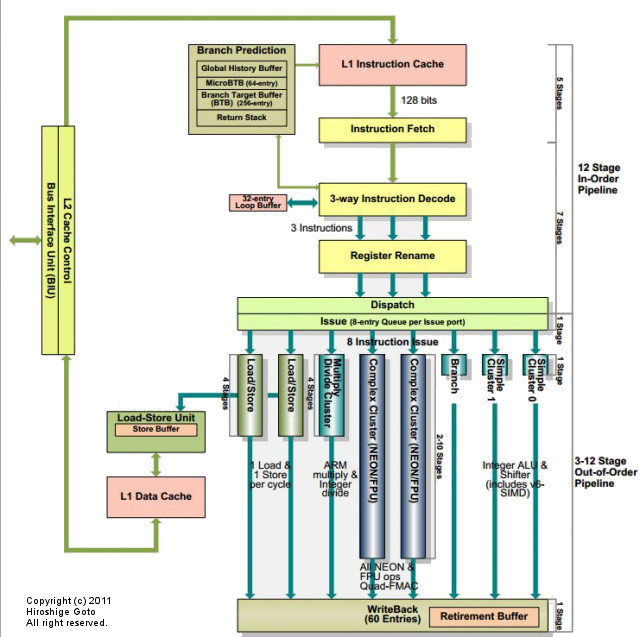
\includegraphics[width=1\textwidth]{img/Cortex_A15_Block_Diagram.jpg}
		\caption{Cortex A15 Block Diagram \cite{sloss2004arm}}
		\label{fig:blockdiagram}
	\end{figure}

	In our cache oriented obfuscation method, we have assumed the system which we worked on is Von Neumann so far. In our implementation, we showed deobfuscation code routine in listing\ref{code:obfuscation}. The reason why we can not simply implement this model is, it is working on the instruction section which actually stored in instruction cache, but in Modified Harvard architecture, there is no direct access to write instruction caches. As seen in figure \ref{fig:blockdiagram}, after fetching obfuscated instruction code into data cache and deobfuscation and storing it back to the cache, it does not move directly to instruction cache. It has to be evicted back to main memory and be fetched into instruction cache instead. Therefore, if we implement same code on Modified Harvard architecture, we encounter with incoherent cache issue which obstructs deobfuscation of instruction or we cause to leak our plain code to upper layer memory. If there is one more layer cache such as L2 cache, instruction and data cache communicate over those; however, it reduces our attack's stealthiness in any case.

\section{Solution}
	In brief and on the whole of mentioned issue in the previous section is the obstacles of modifying instruction cache's values. to sum up our issue, we have two caches which are "dcache" which we can read and write but can't not execute and "icache" which we can execute but can't read\footnote{we can't read it directly, but we can observe its results and estimate it.} and write, thereby we can not deobfuscated and run obfuscated code in the same cache. The question we answered in this section is whether it is possible to redesign a running program's control flow in support of data which it is working on or not. It is only possible, when we design instructions and  statements in the program depending on the branches, namely values that branches depending on. In computer science convention, some methods of interpretation is equivalent to our definition and requirement, and it is shoved that the ability of the interpreter can be equal to ability of the machine it is working on\cite{mak2011writing}\cite{abelson1996structure}. Even though it is possible to building our own interpreter, it is not recommended, because it will be embedded in "Icache" which is plain text and possible to identifying and obtaining signatures. Therefore, we propose to use well known interpreter; then, it could be legalized on signature detection phase.

	\subsection{Flying over Interpreter}
	Instead of running a machine code on target system, we proposes interpreting byte codes or structured abstraction (and therefore it is not bound to any specific machine code but the interpreter itself) for Harvard architecture system. It makes malware architecture independent(On the other hand, it is still cache dependent malware) except stub part. Although Interpretation and compilation are two different methods, they are tightly coupled terms in computer programming. Hence, they are not mutually exclusive on implementation of high level language. Interpreted or compiled languages mean the canonical implementation of the language is compiler or interpreter based\cite{mak2011writing}.

	There are typically several variants of interpreters in a spectrum between compiling and interpreting\cite{mak2011writing}. Byte code interpreting is a method for parsing code directly from interpreter language to byte code. The byte code is not machine code for specific architecture, but machine code for the interpreter's virtual machine. The byte code representation of the corresponding code is generally highly compressed and optimized because they uses all compilation techniques and backgrounds, but efficiency depending on the interpreter and architecture relationship\cite{mak2011writing}. The second variant of the interpreters is using intermediate representation of interpreter's source code. Concrete and abstract syntax tree interpreters are the two of the most known and acknowledged examples. It has more overhead than byte code representation, but it is easier to interpret and preform better analysis during runtime because of better structure and relation representation between statements of the code\cite{mak2011writing}. The one of another variant is just-in-time compilation. They are not pure interpreters or compilers. This techniques compile byte code or intermediate representation to the native code at runtime. Therefore, it is not appropriate for our methods to use because it is still compilation and running native code directly. 

	In figure \ref{fig:blockdiagram}, our approach is illustrated. In this example, there is one shared memory, one "Icache", one "Dcache" and one CPU. It is a part of the whole system, and we assume there are more nodes connected to the same shared memory, but only one of the nodes showed in figure. Stub section of the Icache inherited from the previous chapters. Basically, it deobfuscates body of the malware  which is stored in dcache. As we can load, process and store values to dcache, stub implementation and internals are same. However, when we need to run the deobfuscated code on dcache, we use interpreter to bypass the obstacle, in contrast to previous proposals. Feeding interpreter from memory has already been supported by most of the interpreters for embedded devices e.g. Python, Forth, Basic interpreters. The only thing they need generally starting address. In addition to previous proposals, after running body of the malware, obfuscation could be handled by interpreter at the end of the gadget, or a tail section must be added, after interpreter code in Icache. 
	


	\begin{figure}[h!]
	\centering
	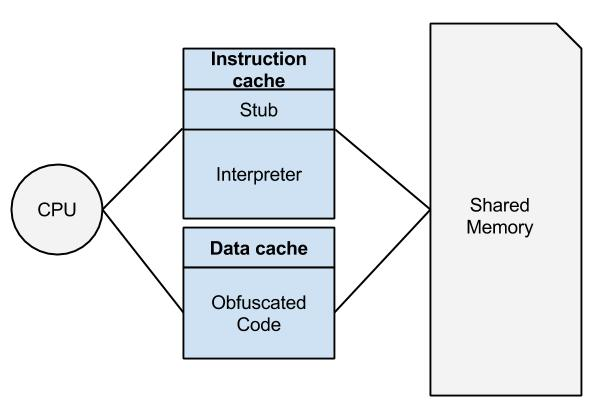
\includegraphics[width=1\textwidth]{img/Harvard_implementation.jpg}
	\caption{Illustration of Our Approach}
	\label{fig:blockdiagram}
	\end{figure}

	\subsection{Forth Interpreter Language}
		Forth programmers traditionally pay importance and emphases complete understanding and control over the machine and its architecture. Therefore, first principle of Forth is simplicity and openness, and it is completely documented and clearly easy designed. Koopman says in 1993 "Type checking, macro preprocessing, common subexpression elimination, and other traditional compiler services are feasible, but usually not included in Forth compilers and this simplicity allows Forth development systems to be small enough to fit in the on-chip ROM of an 8-bit microcontroller. On the other hand, Forth's extensibility allows "full-featured" systems to consume over 100K bytes and provide comprehensive window-based programming environments."\cite{koopman1993brief}, and it is more than fit for recent systems. This simplicity is one of the most important reason why we choose it for our implementation, but the most important reason, it gives you full control between compilation and interpretation. Beside, it is also designed for the embedded systems which use ROM memory instead of ICache, but similarly with our approach, it is read only memory, so it is treasury for our approach. 

		Because there is no explicit Forth parser and no formal grammar, it does not have many concrete standard. There are a few words with ANS Fort which are compiled in assembly, so it is quite simple and small. Moreover, Fort interpreter is very elastic to implement assembly words or remove them, but the standard forth interpreters are better options in term of stealthiness. 

		There are two level of interpretation in Forth, which are text and address interpreting\cite{koopman1993brief}. While text interpreting accepts keyboards or file inputs, address interpreting accepts memory inputs. Text interpreter mode parse white-space separate character string and determine their role in the process. First, it checks whether extracted string is word or not. if it is a word; then, do interpret word's statements, else it checks whether number or not. if it is number then push it to stack, else return exception. It is main control flow of the Forth text interpretation\cite{pelc2011programming}. On the other hand, address interpretation is a bit more complex. It used to execute Forth words which are actually dictionary structures. They all stitched each other with address pointers, and ultimately they point assembly word which is mentioned above and embedded in Forth interpreter. Therefore, there are a few root words which are written in assembly and children words which point parents and ultimately roots. 

\todo[inline]{Add an example code}
\section{Pitfalls and Fallacies}
	In this chapter, we do not concern the difficulties arise from cache coherency mechanism and we worked on incoherent caches. It is probable to implement "flying over interpreter" method with timing attack approach, but there is much more complexity on implementation phases. However, it theoretically has same principles. During implementation of stepped control flow, there could be more overhead related to interpretation. When we need to calculate interpretation latency, we should consider algorithmic overheads. The code which is processed by interpreters frequently uses threaded code. Threaded code refers to implementation of call routine and their consistence. We should also consider the latency which is arising out of this threaded code overhead, and prefer proper algorithms to decide interpreter. 

	Throughout this chapter, we never modified the values in instruction chapter, which is the head of our gadget and involve with an interpreter and stub parts. In order to prevent misunderstanding, it is better to underline that we can modify the values in the instruction cache, but if we move values from the data cache to instruction cache, it will lose its stealthiness, but not vice verse. Therefore, we can move instruction cache values in the data cache and modify them freely. It gives us an ability to regenerate stub part again and again.

	Abstract syntax tree method as an intermediate interpretation language is pretty compact and compressed representation of byte codes\cite{kistler1999tree}, but produce more overhead\cite{garen2008announcing}, so it is better to use it systems without cache coherency. Also, code density can vary from compilation method to method. Because we have limited space, it is better to fit as much as code in minimum space. Due to the division of data and instruction caches, Harvard systems have half sized cache for data.
\chapter{Conclusion and Further Works}
\bibliographystyle{gucmasterthesis}
\bibliography{gucmasterthesis}
\appendix
\chapter{Cache Memory Simulation}
\begin{verbatim}
__author__ = 'caglar'
import random


class Memory(object):
    def __init__(self):
        self.memory = {}

    def __getitem__(self, item):
        try:
            return self.memory[item]
        except KeyError:
            return 0

    def __setitem__(self, key, value):
        self.memory[key] = value


class Cache(object):
    def __init__(self, size=32768, block_size=64, sets=2):
        self.size = size
        self.block_size = block_size
        self.sets = sets
        self.addr_size = 32
        self.cache = list()
        self.line = size / (sets * block_size)
        self.block_addr_len = self.__calculate_addr_len(self.block_size)
        self.line_addr_len = self.__calculate_addr_len(self.line)
        self.tag_addr_len = self.addr_size - self.block_addr_len - self.line_addr_len
        self.super = None
        self.__build()

    def __repr__(self):
        return str(self.cache.__len__())

    def __getitem__(self, address):
        query = self.toquery(address)
        return self.read_request(query)

    def __setitem__(self, address, value):
        self.write_request(address, value)

    def setsuper(self,super):
        self.super = super

    def __build(self):
        for i in range(self.line):
            self.cache.append(CacheLine(i, self.block_size, self.sets))

    def __calculate_addr_len(self, size):
        i = 0
        result = 1
        while size > result:
            result <<= 1
            i += 1
        return i

    def toquery(self, address):
        mask = (1 << 32) - 1
        query = {"address": address,
                 "tag": address >> (self.addr_size - self.tag_addr_len),
                 "index": (address >> (self.block_addr_len)) << ((self.addr_size - self.line_addr_len) & mask) >> (
                     self.addr_size - self.line_addr_len),
                 "block": ((address << (self.addr_size - self.block_addr_len)) & mask) >> (
                     self.addr_size - self.block_addr_len)}
        return query

    def isvalid(self, query):
        for i in range(self.cache[query["index"]].sets):
            if (self.cache[query["index"]].lines[i]["tag"] is query["tag"]) and (self.cache[query["index"]].lines[i]['valid'] is True):
                self.cache[query["index"]].used = i
                return self.cache[query["index"]].lines[i]
        return False

    def read_request(self, query):
        line = self.isvalid(query)
        if line:
            return self.__read_hit(line, query)
        else:
            return self.__read_miss(query)

    def __read_hit(self, line, query):
        return line["data"][query["block"]]

    def __read_miss(self, query):
        self.request_line(query) #proof it later.
        return self.read_request(query)


    def write_request(self, address, value):
        query = self.toquery(address)
        line = self.isvalid(query)
        if line is not -1:
            return self.__write_hit(line, query, value)
        else:
            return self.__write_miss(query)

    def __write_hit(self, line, query, value):
        line["data"][query["block"]] = value
        line["dirty"] = True

    def __write_miss(self, query):
        pass

    def request_line(self, query):
        line = query["address"] - query["block"]
        rline = {"tag": query["tag"], "data": bytearray(self.block_size)}
        for i in range(self.block_size):
            rline["data"][i] = self.super[line+i]
        self.cache[query["index"]].fill_line(rline)


class CacheLine(object):
    #CacheLine is a Class for defining each cache blocks in cache hierarchy
    #During initialization it build a static block of given sets sized array with given block size as byte
    #It has only one method to fill remote block in.
    def __init__(self, index, size, sets):
        self.size = size
        self.sets = sets
        self.index = index
        self.lines = list()
        self.__build()
        self.used = 0

    def __repr__(self):
        return repr(self.lines)

    def __build(self):
        #Initialize the first view of the cache.
        #It will invoke build_line() for each line of the cache.
        for i in range(self.sets):
            self.lines.append(self.__build_line())

    def __build_line(self):
        #Build a line with default variables.
        #data is a byte array which is given length with size
        data = bytearray(self.size)
        return {"tag": 0, "valid": False, "dirty": False, "used": False, "data": data}

    def mark_used(self, line):
        self.used = line

    def give_replaceable(self):
        if self.sets == 1:
            return 0
        else:
            line = random.randint(0, self.sets - 1)
            if self.used != line:
                return line
            else:
                return (line + 1) % self.sets

    def fill_line(self, rline):
        # It fills the corresponding block from the upper layer into the line .
        # Input "rline" is abbreviation of remote line formed as {tag, data}
        # As default, it uses Not recently used, random replacement Policy
        i = self.give_replaceable()
        self.lines[i]["tag"] = rline["tag"]
        self.lines[i]["valid"] = True
        self.lines[i]["dirty"] = False
        self.lines[i]["data"] = rline["data"]
\end{verbatim}
%!TEX root = thesis.tex
\chapter{Real Systems Cache Coherency Latency Simulation Results}
\section{Small Topology}
\subsection{Small Topology Simulation with Two Percent Injection Rate Configuration File and Results}
\lstinputlisting{small_02.txt}
\subsection{Small Topology Simulation with Four Percent Injection Rate Configuration File and Results}
\lstinputlisting{small_04.txt}

\section{Crowded Topology}
\subsection{Crowded Topology Simulation with Two Percent Injection Rate  Configuration File and Results}
\lstinputlisting{crowded_02.txt}

\end{document}

